%  LaTeX support: latex@mdpi.com 
%  For support, please attach all files needed for compiling as well as the log file, and specify your operating system, LaTeX version, and LaTeX editor.

%=================================================================
\documentclass[preprints]{Definitions/mdpi} 
% For posting an early version of this manuscript as a preprint, you may use "preprints" as the journal and change "submit" to "accept". The document class line would be, e.g., \documentclass[preprints,article,accept,moreauthors,pdftex]{mdpi}. This is especially recommended for submission to arXiv, where line numbers should be removed before posting. For preprints.org, the editorial staff will make this change immediately prior to posting.

%--------------------
% Class Options:
%--------------------
%----------
% journal
%----------
% Choose between the following MDPI journals: languages  

%---------
% article
%---------
% The default type of manuscript is "article", but can be replaced by: 
% abstract, addendum, article, book, bookreview, briefreport, casereport, comment, commentary, communication, conferenceproceedings, correction, conferencereport, entry, expressionofconcern, extendedabstract, datadescriptor, editorial, essay, erratum, hypothesis, interestingimage, obituary, opinion, projectreport, reply, retraction, review, perspective, protocol, shortnote, studyprotocol, systematicreview, supfile, technicalnote, viewpoint, guidelines, registeredreport, tutorial
% supfile = supplementary materials

%----------
% submit
%----------
% The class option "submit" will be changed to "accept" by the Editorial Office when the paper is accepted. This will only make changes to the frontpage (e.g., the logo of the journal will get visible), the headings, and the copyright information. Also, line numbering will be removed. Journal info and pagination for accepted papers will also be assigned by the Editorial Office.

%------------------
% moreauthors
%------------------
% If there is only one author the class option oneauthor should be used. Otherwise use the class option moreauthors.

%---------
% pdftex
%---------
% The option pdftex is for use with pdfLaTeX. If eps figures are used, remove the option pdftex and use LaTeX and dvi2pdf.

%=================================================================
% MDPI internal commands
\firstpage{1} 
\makeatletter 
\setcounter{page}{\@firstpage} 
\makeatother
\pubvolume{1}
\issuenum{1}
\articlenumber{0}
\pubyear{2022}
\copyrightyear{2022}
%\externaleditor{Academic Editor: Firstname Lastname}
\datereceived{} 
\dateaccepted{} 
\datepublished{} 
%\datecorrected{} % Corrected papers include a "Corrected: XXX" date in the original paper.
%\dateretracted{} % Corrected papers include a "Retracted: XXX" date in the original paper.
\hreflink{https://doi.org/} % If needed use \linebreak
%\doinum{}
%------------------------------------------------------------------
% The following line should be uncommented if the LaTeX file is uploaded to arXiv.org
%\pdfoutput=1

%=================================================================
% Add packages and commands here. The following packages are loaded in our class file: fontenc, inputenc, calc, indentfirst, fancyhdr, graphicx, epstopdf, lastpage, ifthen, lineno, float, amsmath, setspace, enumitem, mathpazo, booktabs, titlesec, etoolbox, tabto, xcolor, soul, multirow, microtype, tikz, totcount, changepage, attrib, upgreek, cleveref, amsthm, hyphenat, natbib, hyperref, footmisc, url, geometry, newfloat, caption

%=================================================================
%% Please use the following mathematics environments: Theorem, Lemma, Corollary, Proposition, Characterization, Property, Problem, Example, ExamplesandDefinitions, Hypothesis, Remark, Definition, Notation, Assumption
%% For proofs, please use the proof environment (the amsthm package is loaded by the MDPI class).

%=================================================================
% Full title of the paper (Capitalized)
\Title{The Categorization of L3 vowels at first exposure by Spanish-English bilinguals}

% MDPI internal command: Title for citation in the left column
\TitleCitation{The Categorization of L3 vowels at first exposure by Spanish-English bilinguals}

% Author Orchid ID: enter ID or remove command
\newcommand{\orcidauthorA}{0000-0001-8227-1370} % Add \orcidA{} behind the author's name
%\newcommand{\orcidauthorB}{0000-0000-0000-000X} % Add \orcidB{} behind the author's name

% Authors, for the paper (add full first names)
\Author{Kyle Parrish $^{}$\orcidA{}}


%\longauthorlist{yes}

% MDPI internal command: Authors, for metadata in PDF
\AuthorNames{Kyle Parrish}

% MDPI internal command: Authors, for citation in the left column
\AuthorCitation{Parrish, Kyle}
% If this is a Chicago style journal: Lastname, Firstname, Firstname Lastname, and Firstname Lastname.

% Affiliations / Addresses (Add [1] after \address if there is only one affiliation.)
\address{Department of Spanish and Portuguese, Rutgers University, New Brunswick, New Jersey, United States\\
}

% Contact information of the corresponding author
\corres{Correspondence: kyle.parrish@rutgers.edu}

%\simplesumm{} % Simple summary

%\conference{} % An extended version of a conference paper

% Abstract (Do not insert blank lines, i.e. \\) 
\abstract{This is the greatest and best abstract in the world.}

% Keywords
\keyword{L3 acquisition; phonetics; multilingualism; perception} 

% added to include csl references 

% The fields PACS, MSC, and JEL may be left empty or commented out if not applicable
%\PACS{J0101}
%\MSC{}
%\JEL{}

%%%%%%%%%%%%%%%%%%%%%%%%%%%%%%%%%%%%%%%%%%
% Only for the journal Diversity
%\LSID{\url{http://}}

%%%%%%%%%%%%%%%%%%%%%%%%%%%%%%%%%%%%%%%%%%
% Only for the journal Applied Sciences:
%\featuredapplication{Authors are encouraged to provide a concise description of the specific application or a potential application of the work. This section is not mandatory.}
%%%%%%%%%%%%%%%%%%%%%%%%%%%%%%%%%%%%%%%%%%

%\datasetlicense{license under which the data set is made available (CC0, CC-BY, CC-BY-SA, CC-BY-NC, etc.)}

%%%%%%%%%%%%%%%%%%%%%%%%%%%%%%%%%%%%%%%%%%
% Only for the journal Toxins
%\keycontribution{The breakthroughs or highlights of the manuscript. Authors can write one or two sentences to describe the most important part of the paper.}

%%%%%%%%%%%%%%%%%%%%%%%%%%%%%%%%%%%%%%%%%%
% Only for the journal Encyclopedia
%\encyclopediadef{Instead of the abstract}
%\entrylink{The Link to this entry published on the encyclopedia platform.}
%%%%%%%%%%%%%%%%%%%%%%%%%%%%%%%%%%%%%%%%%%
\begin{document}

%%%%%%%%%%%%%%%%%%%%%%%%%%%%%%%%%%%%%%%%%%
%% Remove this when starting to work on the template.
%\endnote{This is an endnote.} % To use endnotes, please un-comment \printendnotes below (before References). Only journal Laws uses \footnote.

% The order of the section titles is: Introduction, Materials and Methods, Results, Discussion, Conclusions for these journals: aerospace,algorithms,antibodies,antioxidants,atmosphere,axioms,biomedicines,carbon,crystals,designs,diagnostics,environments,fermentation,fluids,forests,fractalfract,informatics,information,inventions,jfmk,jrfm,lubricants,neonatalscreening,neuroglia,particles,pharmaceutics,polymers,processes,technologies,viruses,vision


\section{Introduction}

Previous research in third language (L3) acquisition has investigated, broadly, how L2 and L3 learning might be distinct.
While some views may subsume L3 learning as another instance of L2 learning, others have advocated for L3 as its own field of study (\citeauthor{flynn_cumulative-enhancement_2004} \citeyear{flynn_cumulative-enhancement_2004}).
One key difference between L2 and L3 learners is their difference in background knowledge prior to learning a new language.
That is, in the case of L2 learning, the learner's first language has been shown to impact the ease of learning a second language, where it appears to be easier to learn languages that are typologically closer than those that are more distant.
A major question concerning L3 research is how language learners who already speak two languages (bilinguals) are impacted by their previously learned languages during acquisition.
Several models have been proposed over the last 15 years which predict this process, and a consensus has yet to be reached.
While some models propose that L3 learners only have access to one of their known languages (either the L2;
\citeauthor{bardel_role_2007} \citeyear{bardel_role_2007}), or the typologically more similar one to the L3 (\citeauthor{rothman_typological_2010} \citeyear{rothman_typological_2010};
\citeauthor{rothman_l3_2011} \citeyear{rothman_l3_2011};
\citeauthor{baauw_cognitive_2013} \citeyear{baauw_cognitive_2013};
\citeauthor{rothman_linguistic_2015} \citeyear{rothman_linguistic_2015}), others suggest that the L3 property in question determines the cross-linguistic (CLI) influence from source languages to the L3, where L3 learners ultimately converge on target-likeness in the event they have an L1 or L2 abstract representation that matches the L3 property being acquired (\citeauthor{westergaard_crosslinguistic_2017} \citeyear{westergaard_crosslinguistic_2017};
\citeauthor{westergaard_microvariation_2021} \citeyear{westergaard_microvariation_2021}; \citeauthor{slabakova_scalpel_2017} \citeyear{slabakova_scalpel_2017}). The present study adds to the body of evidence used to evaluate the predictions of L3 models by recruiting a relatively large sample of bilinguals and monolinguals and exposing them to vowel sounds in an unknown language. The study begins by reviewing the work done in L3 acquisition as a whole, then covers studies done specifically in production and perception.

\hypertarget{background}{%
\subsection{Background}\label{background}}

The models of L3 acquisition were primarily proposed using empircal evidence from studies in the acquisition of morphosyntactic properties of a third language.
Importantly, there is evidence in the literature for all views.
In a recent systematic review of L3 transfer studies, \citeauthor{rothman_review_2019} (\citeyear{rothman_review_2019}) reviewed and coded a total of 92 studies which investigated how the L1 or L2 impacted the L3.
Possible coding categories included a.) typological transfer, in which the L1 or L2 could impact the L3, depending upon which was a closer typological match, b.) hybrid transfer, in which both L1 and L2 influence was observed, c.) L2 transfer, where the L2 impacted the L3 regardless of typology, and d.) L1 transfer.
In any case in which the coders concluded that a potential study could be counted as evidence of more than one category, both were coded as providing evidence for a particular view.
In the results, the authors focused on 82 of the 92 studies which reported the influence from one of the two source languages was unhelpful (caused not target-like performance on a given task).
Of the 82, the most were explained by typological transfer (n = 51), while 23 were explained by L2 status, 18 could be explained by hybrid transfer, and finally 15 could be explained by L1 transfer.

\hypertarget{l3-production-studies}{%
\subsubsection{L3 Production Studies}\label{l3-production-studies}}

Work in L3 phonology has similarly yielded mixed results and most studies to date have focused on L3 production, ranging from L2 influence to L1 influence, and finally to influence of both languages.
In particular, L2 influence has been found to have a greater impact on L3 global accent production (\citeauthor{wrembel_l2-accented_2010} \citeyear{wrembel_l2-accented_2010}), vowels (\citeauthor{kamiyama_acquisition_2007} \citeyear{kamiyama_acquisition_2007}), speech rhythm (\citeauthor{gut_cross-linguistic_2010} \citeyear{gut_cross-linguistic_2010}), and VOT (\citeauthor{llama_influence_2010} \citeyear{llama_influence_2010}).
On the other hand, some studies have found an L1 influence on global accent production production despite L3 proficiency (\citeauthor{cabrelli_amaro_foreign_2012} \citeyear{cabrelli_amaro_foreign_2012}), or in VOT in advanced L3 learners (\citeauthor{llama_revisiting_2018} \citeyear{llama_revisiting_2018}).

Finally, other studies have found evidence that L3 VOT falls between L1 and L2 values
For example, \citeauthor{wrembel_vot_2014} (\citeyear{wrembel_vot_2014}) measured VOT and aspiration in all languages of participants with two different language combinations: L1 Polish, L2 English, and L3 French; (2) L1 Polish, L2 English, and L3 German.
The results showed that each language had a specific stop-value, and that the L3 VOT productions were intermediate, falling between the L1 and L2 values.
Similarly, \citeauthor{wrembel_cross-linguistic_2011} (\citeyear{wrembel_cross-linguistic_2011}) examined thirty-two learners of L3 French with L1 Polish and L2 English who were recorded reading lists of words in carrier phrases.
As in previous studies (e.g., \citeauthor{wrembel_vot_2014} \citeyear{wrembel_vot_2014}), combined transfer from the L1 and the L2 in VOT productions was found.
Findings of combined L1 and L2 influence in VOT productions were also reported by \citeauthor{wunder_phonological_2010} (\citeyear{wunder_phonological_2010}) in L3 Spanish speakers, and by \citeauthor{blank_transferencia_2009} (\citeyear{blank_transferencia_2009}) in L3 English speakers who spoke L1 Brazilian Portuguese and L2 French.

The source of this variety of findings in the research is not yet clear.
One possible cause is the risk for sampling error that is associated with low sample studies (\citeauthor{brysbaert_power_2020} \citeyear{brysbaert_power_2020}).
That is, when sample size is low, as it has been in many studies on multilingualism, the likelihood of a proposed difference between groups being due to a false positive result increases.
In other words, differences observed in small groups may have to do with the differences in individual participants more than it does the difference in their underlying group membership.

Following the suspicion that intermediate values might have to do with either sampling issues or proficiency effects, \citeauthor{parrish_l3_vot_2022} (\citeyear{parrish_l3_vot_2022}) examined Mexican Spanish-English bilinguals who produced voiceless stop-initial French words in isolation at first exposure to the language.
The results found that the relative VOT of the L3 fell between their own L1 and L2 values, in line with previous research, and that suggested that intermediate values were less likely to have been seen in previous studies as a result of small samples or proficiency effects.
However, a subsequent analysis of the data suggested that wide individual variation existed, in which some participants produced L3 French as L1 Spanish like, and other produced intermediate, L2-like values.
This result suggests that higher samples could reveal group trends and provide better insights into individual variation in crosslinguistic influence, as opposed to assuming that a single group trend exists.\\
It is unclear whether the trends seen in production might also be found in perception.
By carrying out perception studies, it is possible to examine whether the predictions of L3 models apply more generally to L3 phonoglocial acquistition

\hypertarget{l3-perception-studies}{%
\subsubsection{L3 Perception Studies}\label{l3-perception-studies}}

Even fewer studies have been carried out in L3 perception.
To the author's knowledge, only two studies thus far have investigated the categorization of L3 vowels and have both focused on school age (12-14 year old) bilinguals. (\citeauthor{balas_non-native_2018} \citeyear{balas_non-native_2018}; \citeauthor{wrembel_extending_2019} \citeyear{wrembel_extending_2019}).
\citeauthor{wrembel_extending_2019} (\citeyear{wrembel_extending_2019}) examined the categorization and discrimination of L3 vowels by 10 young trilinguals who spoke L1 German-L2 English-L3 Polish.
To test categorization, a cross-linguistic similarity task was used in which participants heard minimal pairs of sounds and had to rate how similar sounds were on a 1-7 Likert scale.
The results showed evidence that participants assimilated L3 sounds to both L1 and L2 categories, but preferred the L2.
In a second experiment, and AX discrimination task was given to participants to evaluate whether retroflex and palato-alveolar silibant discrimination, a feature of Polish, could be accessed in L3 words.
The results revealed that discrimination of the L1 Polish contrast was very good (84\% accuracy), suggesting that L3 learners retain access to L1 sound contrasts in L3 words.
Additionally, this language specific phonetic discrimination was attended to by even L3 beginners.
\citeauthor{balas_non-native_2018} (\citeyear{balas_non-native_2018}) also used the PAM as a perceptual framework to work in and adapted it to L3 learners.
The study recruited three groups of Polish L1 speakers, including two L3 groups (L1 Polish-L2 English-L3 Dutch and L1 Polish-L2 English-L3 Dutch).
The third group spoke only English as an L2.
All three groups were listened to Dutch vowels and were asked to categorize them given Polish vowel categories.
The L3 groups were not given L2 English categories as options during this task, so the results of this study cannot directly provide evidence that L3 learners categorize L3 sounds using both the L1 and L2 categories.
The same study also conducted an AXB discrimination task of 8 Dutch vowels and found that discrimination was at ceiling for all vowels involved.

\hypertarget{the-present-study}{%
\subsection{The Present Study}\label{the-present-study}}

Building on this work, the present study adapts methods commonly used in studies in L2 bilingual phonology to investigate how the phonetic vowel categories of adults language learners impact their categorization of unknown language vowels near first exposure.
In particular, methods are adopted from studies which have tested the predictions of the Perceptual Assimilation Model for L2 learners (PAM-L2; \citeauthor{bohn_nonnative_2007} \citeyear{bohn_nonnative_2007}).
The model predicts that perception drives L2 phonological acquisition, and that, broadly, the (dis)similarity between sound contrasts in the L1 and L2 predicts how difficult the acquisition of a particular phoneme will be for the learner.
To test these predictions, speakers of a particular language are asked to categorize sounds in a language that they do not speak given the categories of their native language.
The present study presented similar tasks to those used in L2 studies, but included both L1 and L2 categories.
Here, a fully combined design of Spanish-English bilinguals (i.e.~two bilinguals groups and two monolingual groups will be exposed to the same languages, where the bilingual groups have the opposite order of acquisition but know the same languages) categorized vowel sounds in both French and German.
Importantly, all the participants in the present study did not speak French or German.

The languages of French and German were chosen as L3s since they correspond historically to Spanish and English respectively.
Spanish and French are both Romance languages and German and English are both Germanic.
This historical relationship likely corresponds to global typological similarity between these language pairs, and the present design includes vowel conditions (e.g., /i/, which is present in all languages in the current study), which arguably allow for a bias to be observed.
That is, if participants categorized the L3 sound /i/ in L3 French as Spanish-like more often than English like, and the the L3 sound /i/ in German as English-like more often than Spanish-like, despite the acoustic overlap in the stimuli, this would be interpreted as evidence for bias based on global typological effects as the Typological Primacy Model would predict.
Additionally, the vowel spaces of the chosen languages varies sufficiently to create 4 scenarios, which are operationalized in the vowel conditions covered in more detail in the method section of this paper.
Specifically, a situation is created in which the a sound is present in all 4 languages, in Spanish-only, German and French only, in English, German and French only, and in German and French only.

In addition, the present design is novel in that it allows for a within-subjects comparison of the same individual at the initial state of learning to distinct L3s.
This situation is helpful in determining how source languages impanct an L3 in the similar ways that the group design, since it allows for an additional window into whether typological effects (which are operationalized here as acoustic similarity of the vowels cross-linguistically) or order of acquisition better predict categorization patterns in a new language.
Examining L3 learners at first exposure offers at least two advantages.
First, acquisition and influence can better be teased apart when perception is target-like, and second a larger sample can be recruited in which L3 input can be better experimentally controlled for.
As opposed to traditional L3 studies, where participants are actively learning a third language and may vary in L3 proficiency, exposure to input and daily L3 use, absolute beginners have almost no exposure to the L3 in a learning setting.
As a result, initial exposure learners are an ideal population to examine cross-linguistic influence that could not be readily explained by other variables associated with distinct language learning outcomes.
Second, a much larger sample can be recruited, which may strengthen the findings of the present study by reducing the risk of sampling error as a possible cause of the results.

In summary, the present study is guided by the following research questions:

\textbf{RQ1}: Overall, do Spanish-English bilinguals prefer their L1 or L2 when categorizing a new language?

\textbf{RQ2}: Does the L3 that they learn impact their categorization of similar vowel sounds cross-linguistically?

\textbf{RQ3}: When a language is chosen, do bilingual and monolingual speakers differ in their phoneme of choice?

The present study is pseudo-exploratory, in that specific predictions are not made in regard to these research questions.
This is the case due to the lack of comparable studies to date in the literature.
It is important, however, to point out that many L3 models would have specific predictions for these questions.
The predictions will focus here on two of the models: the Typological Primacy Model and the Linguistic Proximity Model (\citeauthor{westergaard_crosslinguistic_2017} \citeyear{westergaard_crosslinguistic_2017};
\citeauthor{westergaard_microvariation_2021} \citeyear{westergaard_microvariation_2021}).
For RQ1, the Typological Primacy Model would predict that global typology should predict either L1 or L2 preference, but this should happen globally at some point in development.
The Linguistic Proximity Model would predict that bilinguals have access to both L1 and L2 sounds, and should largely be helped by the presence of both vowel inventories in L3 vowel perception.

For RQ2, the TPM would predict a difference in categorization as a function of the third language being learned.
That is, it would predict that very similar sounds between two languages (in this case French and German) should be differently categorized.
In particular, global typological relationships should drive the bias of categorizations that are acoustically similar.
On the other hand, The LPM would predict that the sound itself, rather than the language it belongs to, should predict patterns of categorization.
In the present case, the phoneme /i/ is one case which will provide evidence to sort out the predictions of these models.
If, in the both languages and given the phoneme /i/, participants are equally likely to choose and English or Spanish category, it will support the LPM.
On the other hand, if a clear bias can be observed when the phoneme /i/ is played given a particular L3, the TPM would receive support.
For example, if the German /i/ is categorized as English more often than Spanish, this would be taken as evidence of a bias.

For RQ3, the present study will make use of conditional probability to investigate whether, for example, when the Spanish L1 group picks a Spanish category given a particular stimulus, whether they differ from the monolingual groups.
Conditional probability will be calculated by taking the probability of a particular choice and dividing it by the sum of the probability of all of a given language's choices.

\section{Materials and Methods}

\hypertarget{participants}{%
\subsection{Participants}\label{participants}}

A total of 199 participants took part in the present study, after the removal of the data of 10 total participants who self-reported being bilingual yet not feeling comfortable speaking or understanding their second language.
This pool of participants constitutes a mirror image design (\citeauthor{rothman_typological_2010} \citeyear{rothman_typological_2010}; \citeauthor{leung_chapter_2009}, \citeyear{leung_chapter_2009}), in which two bilingual groups who speak the same languages, but have the opposite order of acquisition, are compared.
The present sample includes Mexican Spanish L1-English L2 speakers (n = 59) and English L1-Spanish L2 speakers (n = 55).
The monolingual participants included 29 Mexican Spanish monolinguals and 56 American English speakers.
All participants were recruited online via Prolific.co and were pre-screened to ensure that they were, in the Spanish L1 group, born in Mexico, living in Mexico, and their current IP address suggested that they were in Mexico at the time of the experiment.
Similarly, in the English L1 group, participants were filtered to those who were living in the United States, were born in the United States, and whose IP address suggested that they were in the United States during the time of the experiment.
All participants were also filtered to those who were raised monolingual, but learned a language later in life.
Each participant was compensated for their time taking both the experimental task and the background questionnaire.
Both tasks took a combined total of less than 15 minutes.
In addition to filters in place from Prolfic.co, the participants were screened further using an adapted version of the Bilingual Language Profile cite (\citeauthor{birdsong_bilingual_2012} \citeyear{birdsong_bilingual_2012}).
All participants who answered `no' to the question ``Do you speak a language other than English and Spanish'' were permitted to continue the experiment.

Figure \ref{ao_aoa} represents the self-reported age of onset of L2 learning (panel A), and the first age at which the individual felt comfortable using their L2 (panel B).
As can be seen from the figures, The English L1-Spanish L2 group began L2 learning later on average, while they also felt comfortable in their L2 at a later age than the Spanish L1-English L2 group.

\begin{figure}[H]
\begin{adjustwidth}{-\extralength}{0cm}
\centering
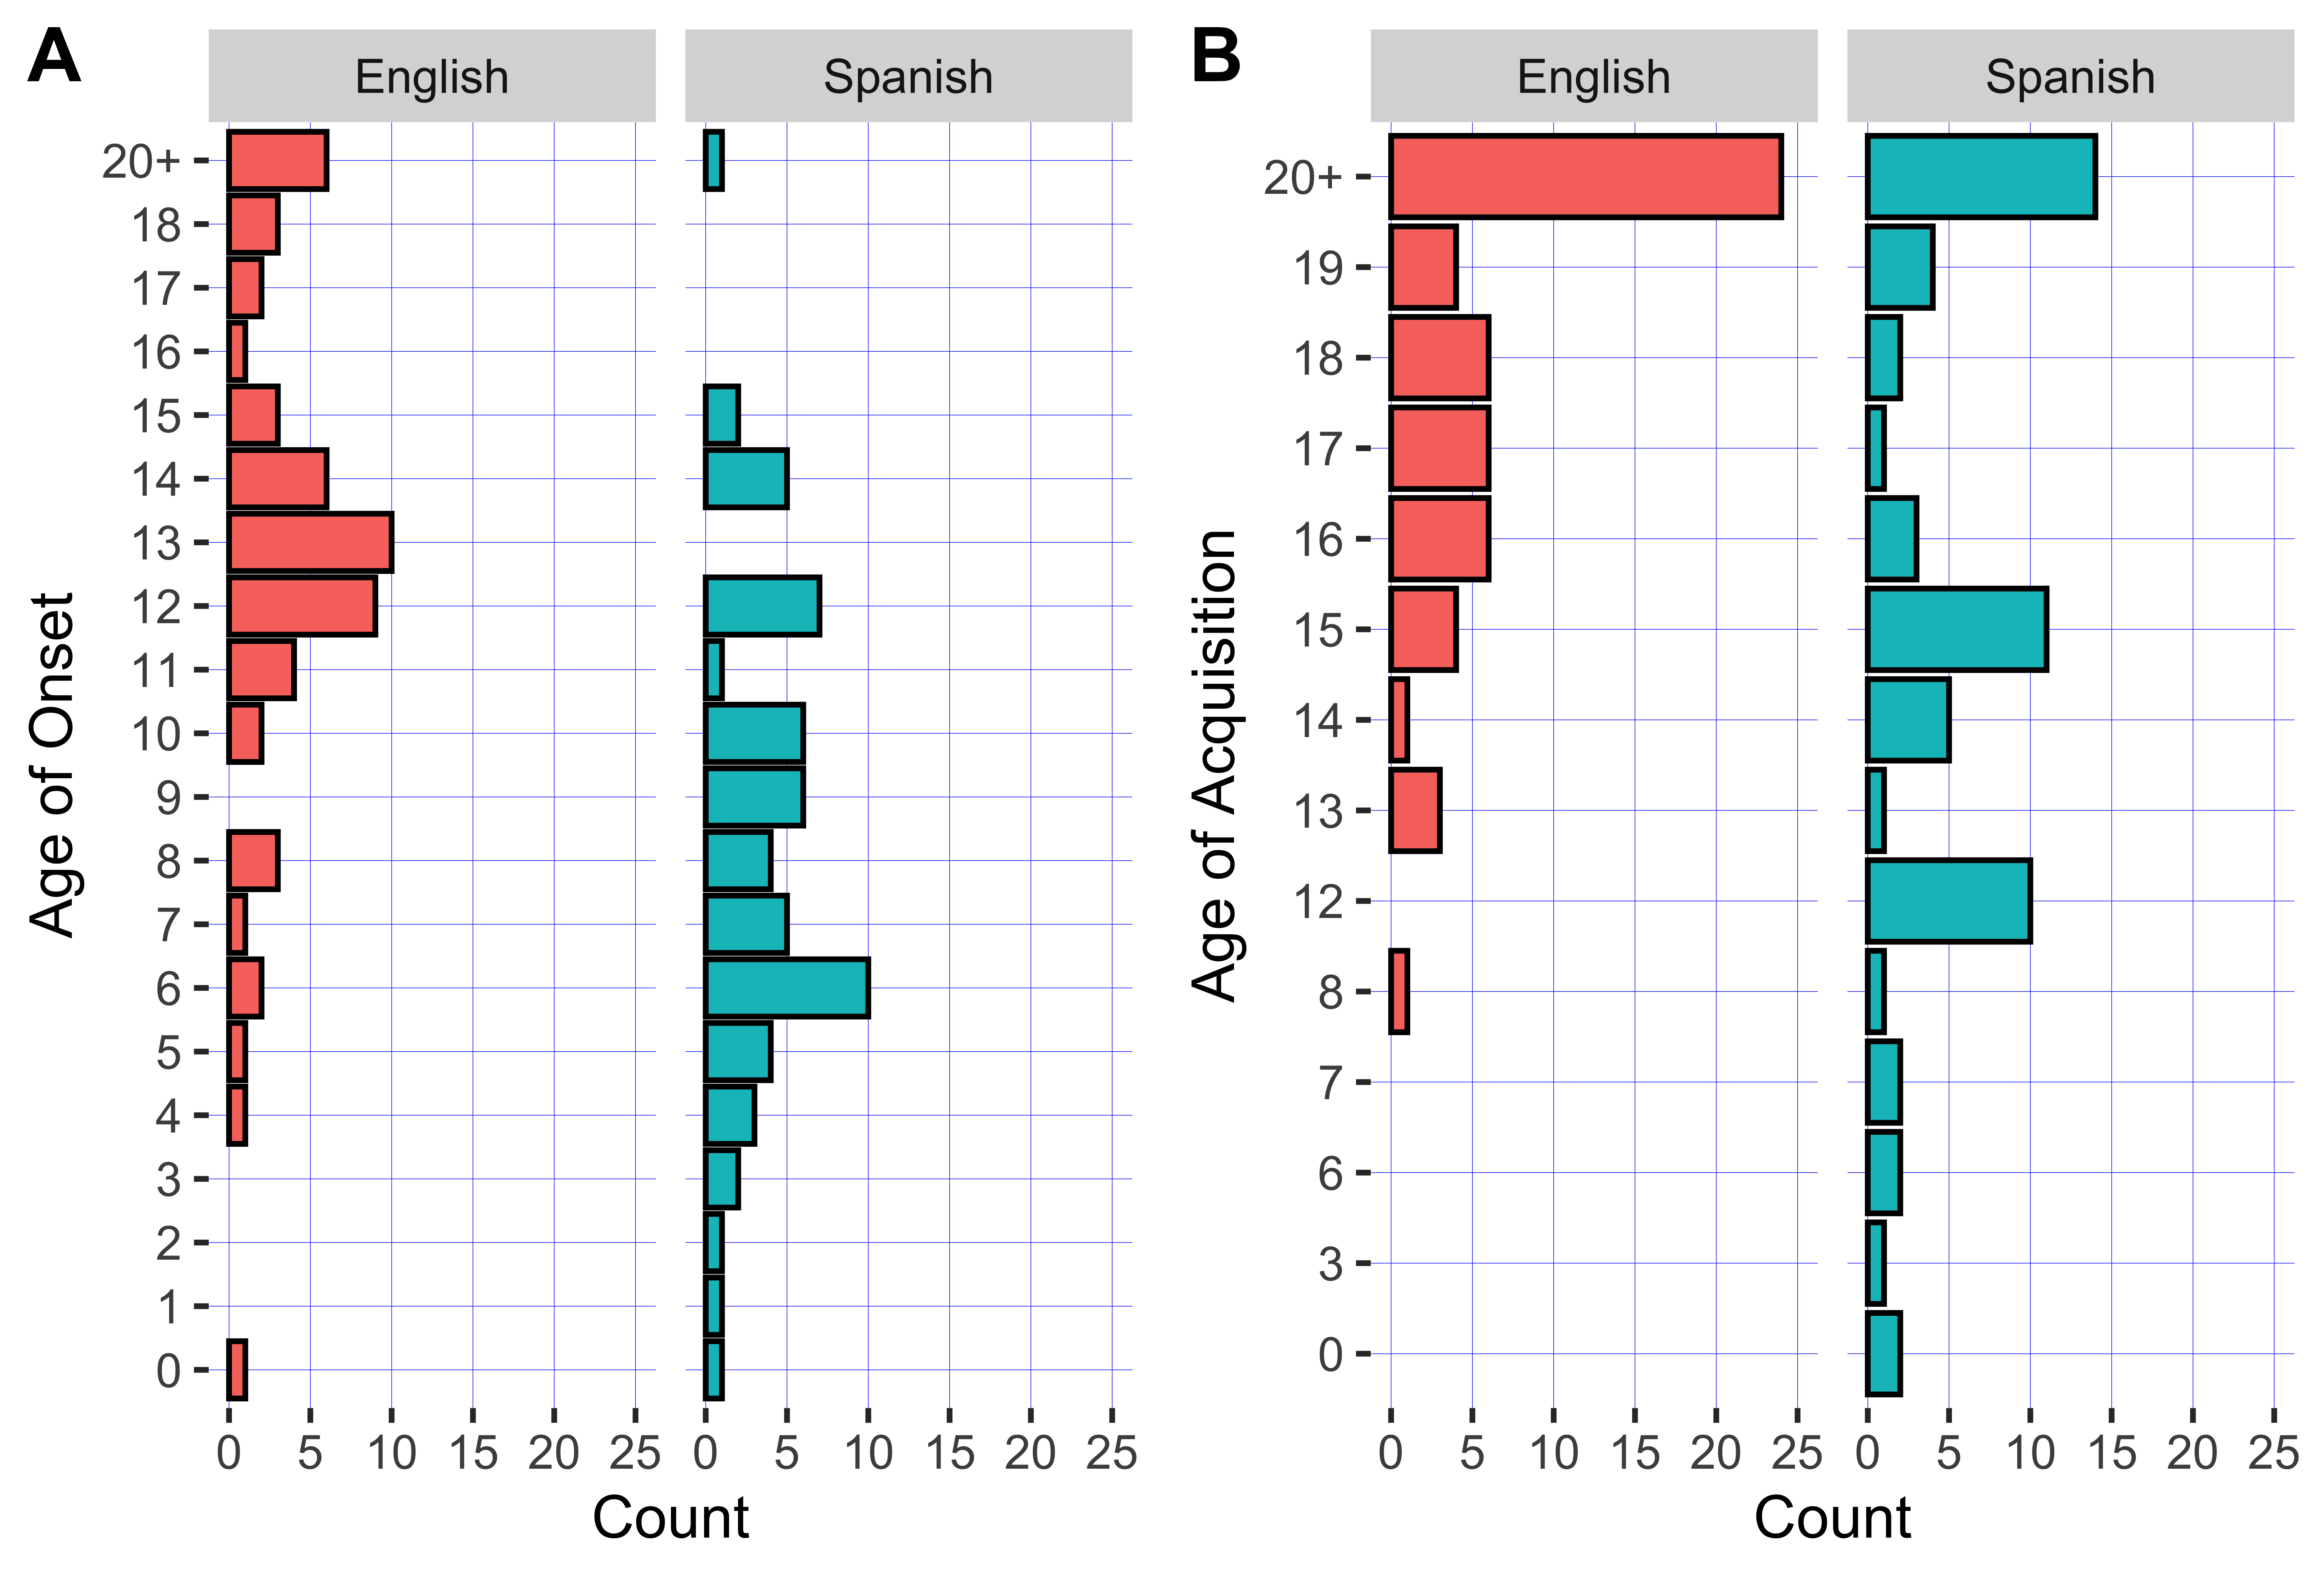
\includegraphics[width=13.5cm]{figs/ao_aoa_combined.png}
\end{adjustwidth}
\caption{(\textbf{a}) Self-reported age of onset of L2 learning, where the panel name represents that participants' L2 (\textbf{b}) Self-reported age of acquisition, in which the participant reported first feeling comfortable in their L2.\label{ao_aoa}}
\end{figure}

The participants also rated their L2 proficiency.
They were given a 0-6 Likert-type scale in which they answered the questions ``How well do you speak {[}their L2{]}?'' and ``How well do you understand {[}their L2{]}?''.
``0'' corresponded to ``not very well at all'', where ``6'' corresponded to ``very well''.

\begin{figure}[H]
\begin{adjustwidth}{-\extralength}{0cm}
\centering
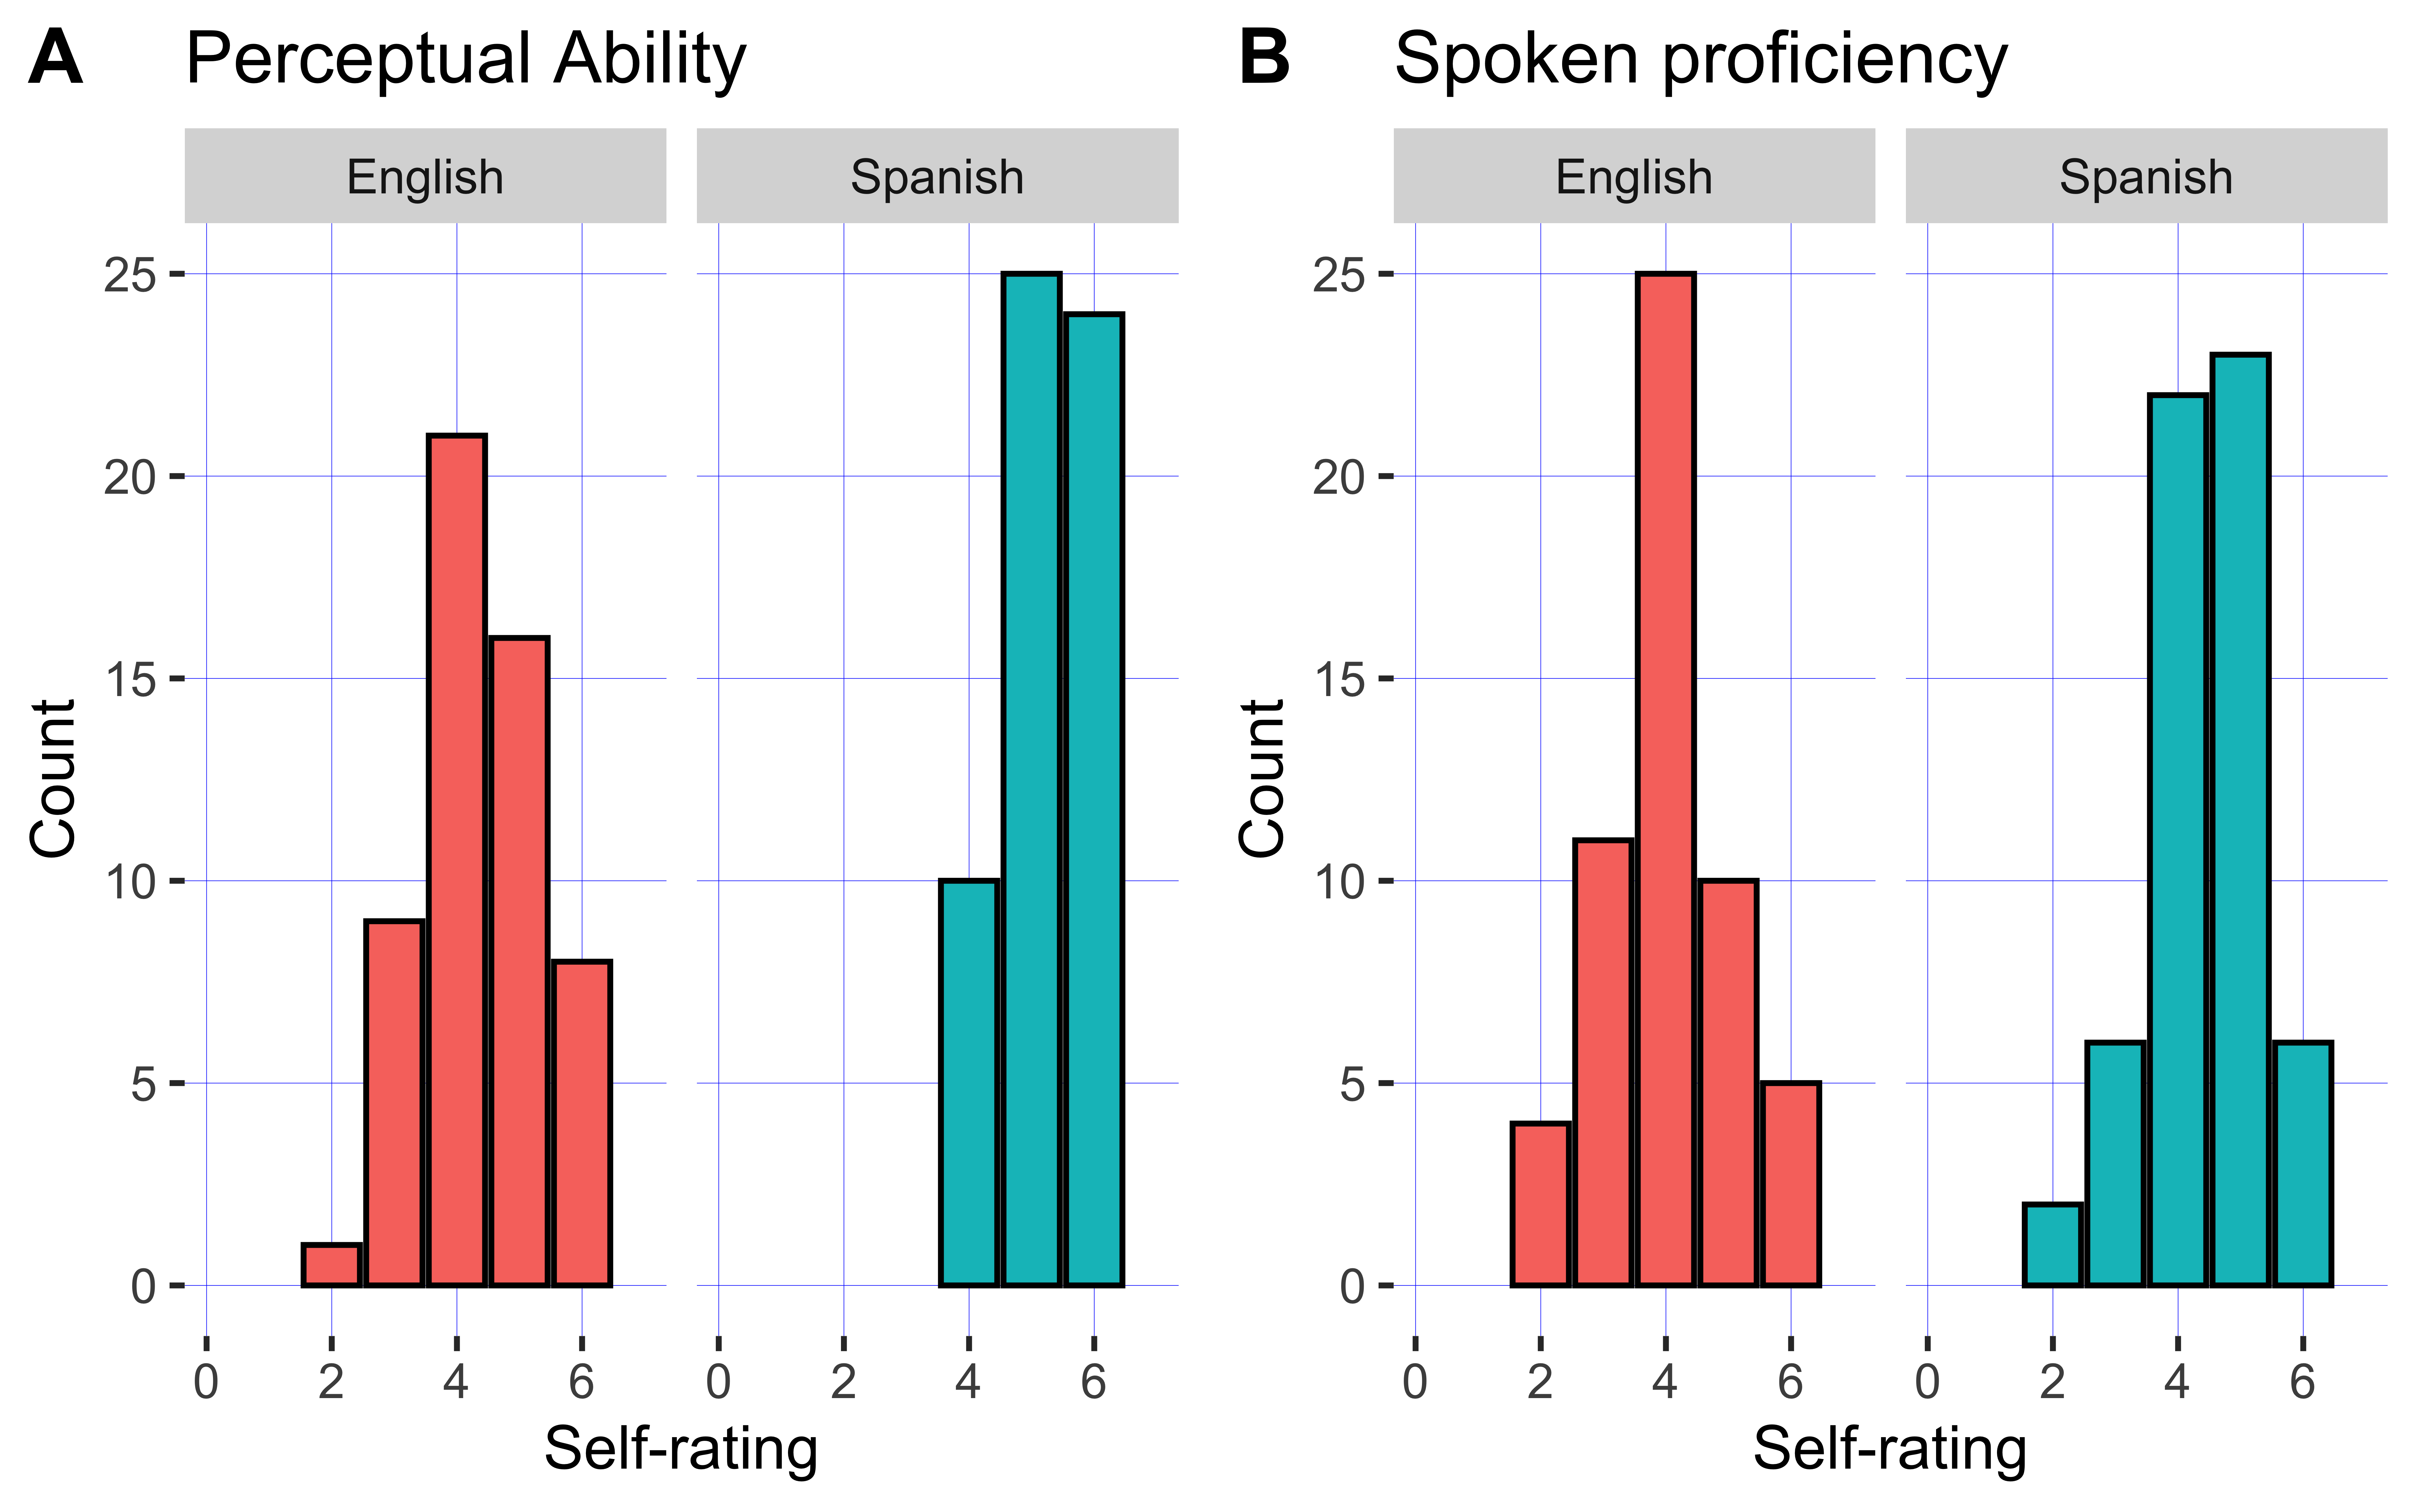
\includegraphics[width=13.5cm]{figs/proficiency_combined.png}
\end{adjustwidth}
\caption{Self-rated L2 Proficiency. The top panels refer to the L1 of the participant and the ratings refer to their L2 (\textbf{a}) Self-rated perceptual ability (\textbf{b}) Self-reported spoken proficiency. \label{fig_prof}}
\end{figure}

Figure \ref{fig_prof} displays the distribution of self-ratings in perceptual ability and spoken proficiency in both groups.
An inspection of this figure suggests that both groups self-rate their perceptual abilities higher than their spoken proficiency, where the Spanish L1 group rated themselves higher overall in both categories.
Specifically, the Spanish group's spoken proficiency was 4.42 (sd = 0.93) and the mean of English self-rated spoken proficiency
was 4.02 (sd = 1.03).
In perception, the Spanish group rated their perceptual abilities at 5.24 (sd = 0.73) on the 0-6 scale, and the mean of English speakers' perceptual proficiency
was 4.38 (sd = 0.99).

\hypertarget{tasks}{%
\subsection{Tasks}\label{tasks}}

All participants completed a total of 3 tasks.
First, all participants completed an adapted version of the Bilingual Language Profile (BLP; \citeauthor{birdsong_bilingual_2012} \citeyear{birdsong_bilingual_2012}) administered using Google Forms.
The profile gathered general background information, including self-rated proficiency and age of onset and acquisition.
Additionally, participants were asked whether they spoke a third language as an added question.
Following the BLP, participants completed two vowel categorization tasks to test their categorization of French and German vowel sounds.
The tasks are similar to those used in studies in L2 bilingual phonology (see, e.g., \citeauthor{bohn_nonnative_2007} \citeyear{bohn_nonnative_2007}; \citeauthor{van_leussen_learning_2015} \citeyear{van_leussen_learning_2015}).

\hypertarget{vowel-categorization-task}{%
\subsubsection{Vowel Categorization Task}\label{vowel-categorization-task}}

The vowel categorization task has been used widely in L2 research, and it broadly intended to provide evidence of the initial state of the L2 phonology.
In these tasks, participants are exposed to sounds in a language that they do not speak and asked to categorize them given their native categories, which are usually given orthographically in carrier words.
The present study mimics this design and adapts it to L3 acquisition, similarly to \citeauthor{wrembel_extending_2019} (\citeyear{wrembel_extending_2019}).
That is, rather than asking participants to categorize sounds using just their native categories, the present study includes both L1 and L2 categories.
During the task, participants first heard a stimulus sound played and then chose a word on the screen that best fit the sound that they heard by pressing the appropriate number key on a keyboard.
Figure \ref{vct} shows the information that participants saw on their screen during the task.
After making each selection, the participants then rated their pick for goodness of fit by clicking a 1-5 continuous Likert scale (Figure \ref{likert}).

\begin{figure}[H]
\begin{adjustwidth}{-\extralength}{0cm}
\centering
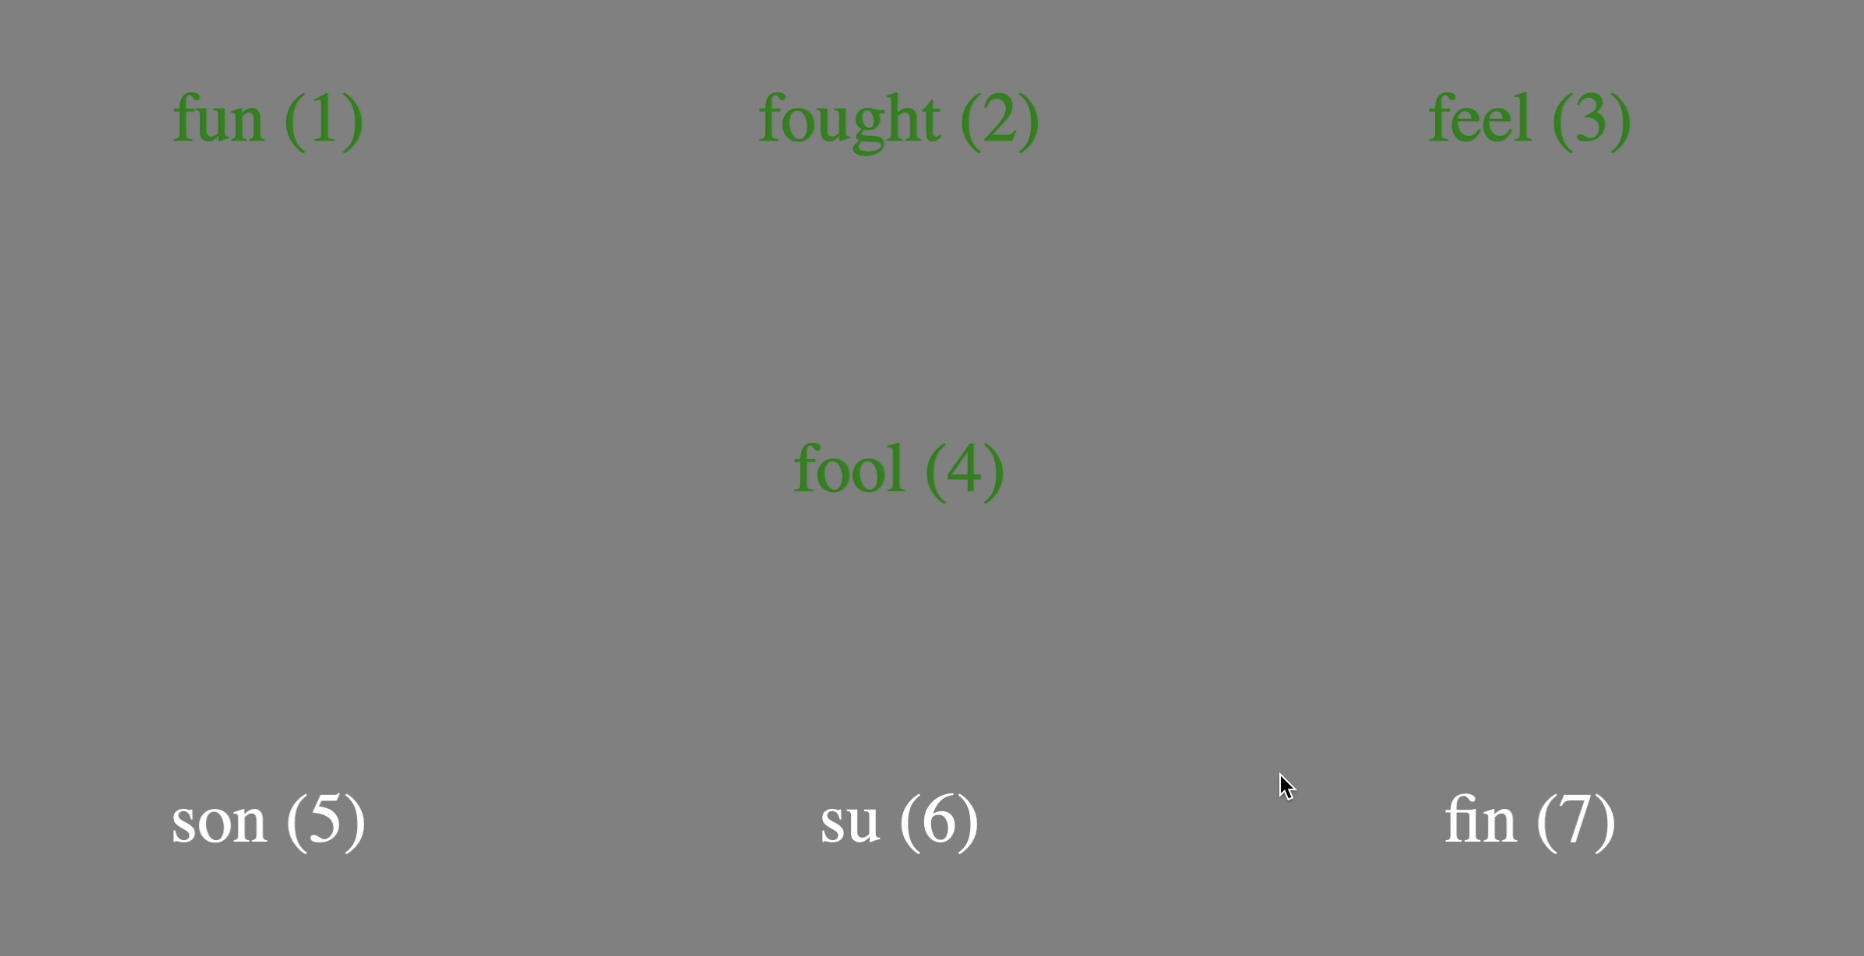
\includegraphics[width=13.5cm]{figs/vct.png}
\end{adjustwidth}
\caption{This is a wide figure.\label{vct}}
\end{figure}

\begin{figure}[H]
\begin{adjustwidth}{-\extralength}{0cm}
\centering
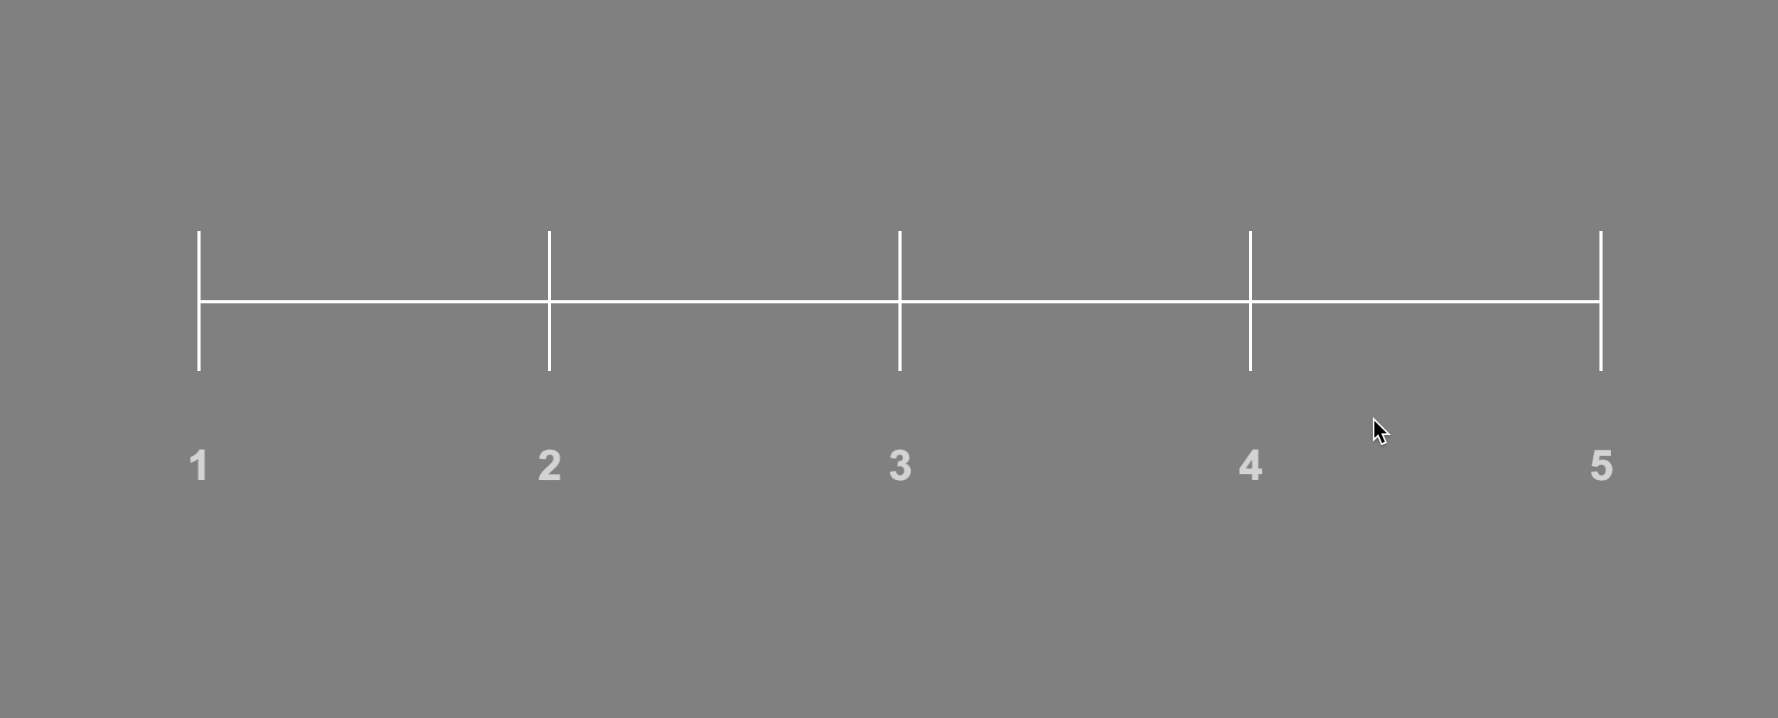
\includegraphics[width=13.5cm]{figs/likert.png}
\end{adjustwidth}
\caption{This is a wide figure.\label{likert}}
\end{figure}

In total, the same four distinct sound conditions were played in both French and German given seven total English and Spanish total categories to choose from.
The vowel sounds included in both experiments were intended to bring about four distinct cross-linguistic situations.
First, the L3 phoneme /i/ was included to create a conflict in which both source languages, Spanish and English, have a similar sound /i/.
The phoneme /i/ was given in the Spanish word \emph{fin} and the English word \emph{feel}.
Next, the L3 phoneme /\^{}\{\}/ was given in an attempt to bias the selection of English.
This condition was intended to be assimilated to the English choice \emph{fun}.
Third, the phoneme /o/ was included to bias the same Spanish category, where a rounded /o/ does not exist in American English.
The intended choice in this case was the Spanish word \emph{son}, but the English word \emph{thought} was also provided as an alternative.
Finally, the phoneme /y/ was added to explore how a sound that is not present in either language will be categorized.
Given that /y/ is a high-front vowel, it is possible that it could be assimilated to other high vowels, either /i/ as in \emph{feel} or \emph{fin}, or /u/, as provided in \emph{fool} or \emph{su}.
The four sounds were embedded in both a fricative /fVf/ and bilibial /pVp/ or /pVf/ frames and played a total of 5 times each.
Thus, each participant categorized 40 tokens per language (5 repetitions x 2 frames x 4 vowel conditions).
The order of the stimuli was counterbalanced and the two tasks were given in a single session with a brief pause between them.
The experiments were programmed in Psychopy (\citeauthor{peirce_psychopy2_2019} \citeyear{peirce_psychopy2_2019}) and made available online via Pavlovia.

The stimuli were recorded by adult, female L1 speakers of French and German respectively and was also collected online.
The speakers were given each vowel in a word or non-word in both a fricative and bilabial frame.
In the event a non-word was provided, a real word containing that vowel sound was included to aid the informant in producing the intended pronunciation of the vowel.
Once the stimuli were recorded, one of the two tokens provided by the speaker for each vowel was selected and re-synthesized adding the appropriate onset and coda.
In total, 8 stimuli were created per language.
Figure \ref{stimuli} shows the formant values of the included stimuli in German and French in comparison to similar sounds in English and Spanish.
For the purpose of this Figure, an adult female speaker of Madrid Spanish and an adult female American English speaker provided vowel tokens of the answer choices in the present study by producing the carrier words while being recorded in PRAAT (\emph{son}, \emph{su} and \emph{fin} in Spanish and \emph{fought}, \emph{feel}, \emph{fool}, and \emph{fun} in English).

\begin{figure}[H]
\begin{adjustwidth}{-\extralength}{0cm}
\centering
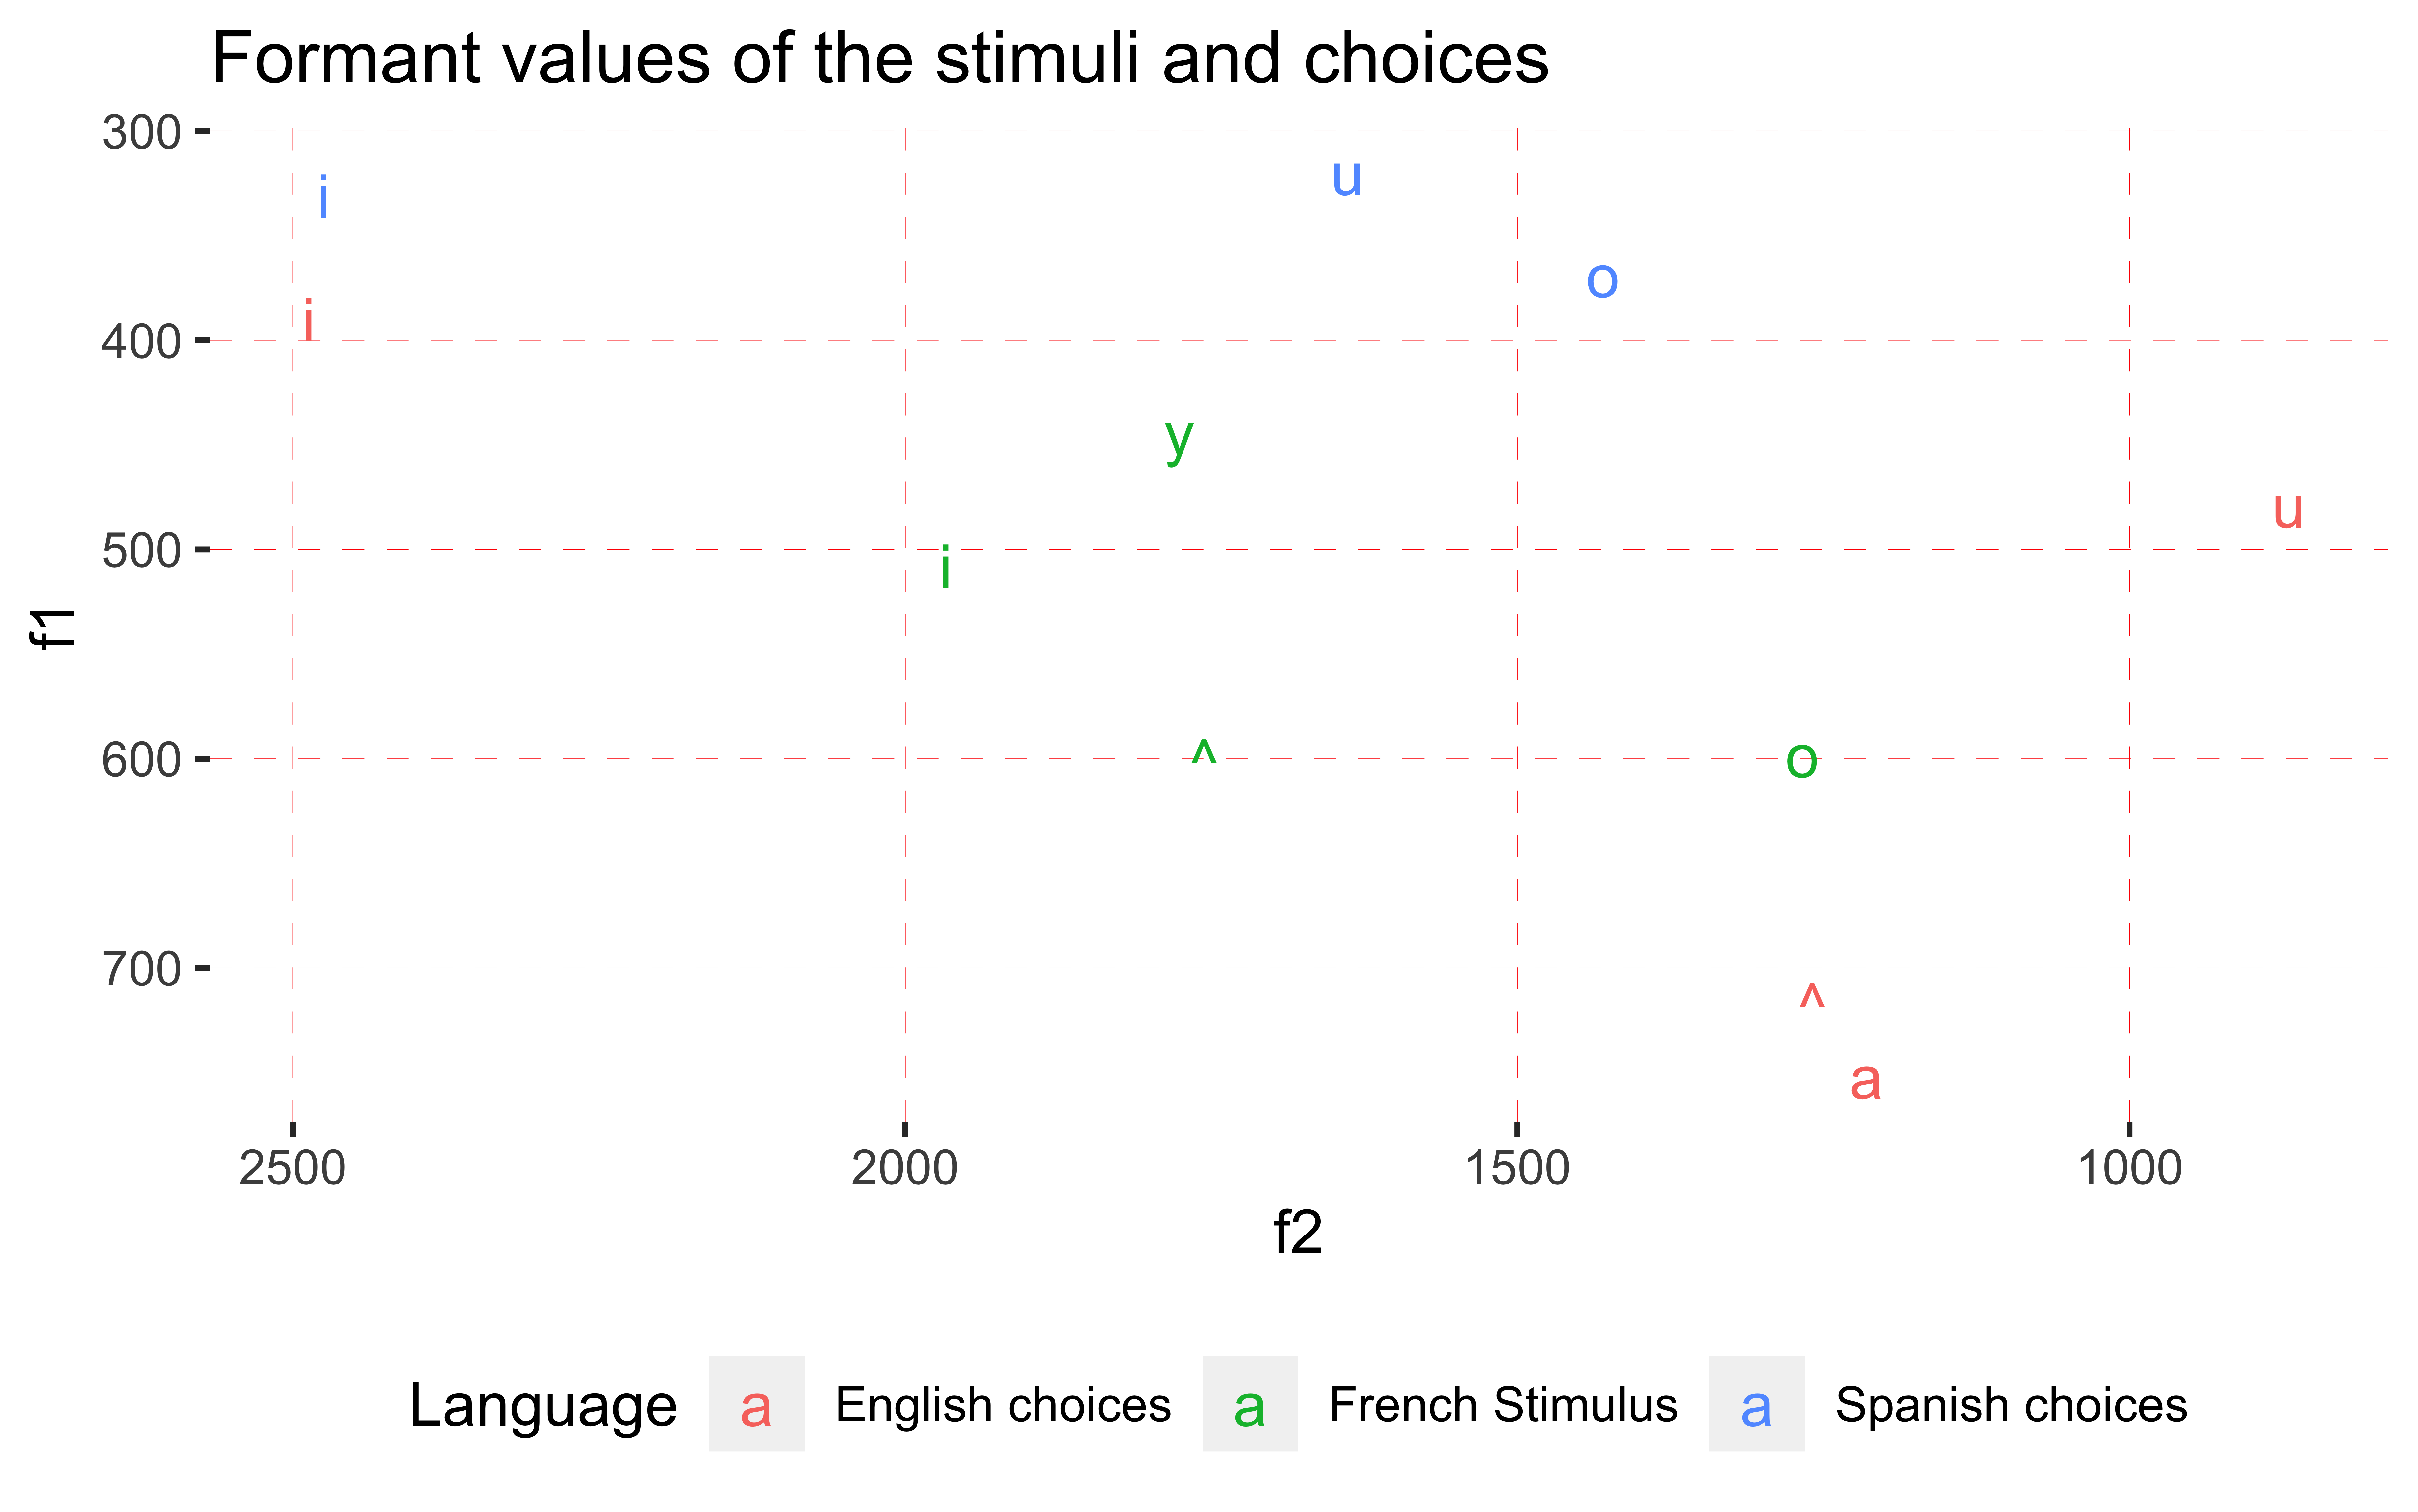
\includegraphics[width=13.5cm]{figs/stimuli.png}
\end{adjustwidth}
\caption{This is a wide figure.\label{stimuli}}
\end{figure}

\hypertarget{procedure}{%
\subsection{Procedure}\label{procedure}}

All participants first completed the adapted Bilingual Language Profile (\citeauthor{birdsong_bilingual_2012} \citeyear{birdsong_bilingual_2012}) online.
An English and Spanish version of the questionnaire was adapted and given to the participants based on their L1.
All participants who answered ``no'' to the question ``Besides English and Spanish, do you speak a third language?'' were invited to take part in the experimental task.
The vowel categorization task was given to participants online. An English and Spanish version of this task was also created, in which all instructions were given in either English or Spanish.
During the task, all participants heard French first, followed by a brief pause, and then heard German sounds.

\hypertarget{statistical-analysis}{%
\subsection{Statistical Analysis}\label{statistical-analysis}}

For the vowel categorization tasks, the data were analyzed using a series of Bayesian multilevel multinomial logistic regression model in R (\citeauthor{R-base} \citeyear{R-base}).
The models were fit using the R package \texttt{brms}
(\citeauthor{R_brms_a} \citeyear{R_brms_a}).
A model was run for each of 4 groups: L1 Spanish, L1 English, monolingual English and monolingual Spanish.
In each model, the outcome variable was word choice.
In the bilingual groups, this consisted of 7 total options (3 Spanish words: \emph{fin}, \emph{su}, \emph{son} and 4 English words: \emph{fun}, \emph{fought}, \emph{feel}, and \emph{fool}.)
Thus, outcome of the bilingual models estimates the log odds of choosing one of the seven choices, and would sum to 1 when converted to probability.
The fixed effect predictors of the bilingual models were phoneme (/i/, schwa, /y/ and /o/), stimulus language (French or German) and Lextale score (continuous and transformed to a z-score) and all higher order interactions. Random effects included a random intercept for participant to take into account the nested structure of the data.

The monolingual models modeled word choice as a function of phoneme and stimulus language, again with a random intercept for participant to take into account the nested structure of the data.
In this case, language choice was more limited in each group limited, with the Spanish monolingual group only having 3 options: \emph{fin}, \emph{su}, \emph{son}, while the English group had 4 word choices: \emph{fun}, \emph{fought}, \emph{feel}, and \emph{fool}.
The model included regularizing, weakly informative priors (\citeauthor{gelman_prior_2017} \citeyear{gelman_prior_2017}),
which were normally distributed and centered at 0 with a standard deviation of 8 for all population-level parameters.
The region of practical equivalence (ROPE) was set to 0.18, as the outcome variable was in log-odds (see \citeauthor{kruschke_rejecting_2018} \citeyear{kruschke_rejecting_2018}).
All models were fit with 2000 iterations (1000 warm-up).
Markov-chain Monte-Carlo sampling was carried out with 6 chains distributed between 8 processing cores.

\hypertarget{results}{%
\section{Results}\label{results}}

\begin{table}[H] 
\caption{The percentage of categorizations of phonemes in the English monolinguals group.\label{el1_fr}}
\newcolumntype{C}{>{\centering\arraybackslash}X}
\begin{tabularx}{\textwidth}{CCCCCC}
\toprule
stim\_language & choice & i & o & schwa & y \\ 
  \hline
German & feel & \textbf{0.93} & 0.01 & 0.01 & 0.06 \\ 
German & fool & 0.02 & \textbf{0.45} &  & \textbf{0.78} \\ 
German & fought & 0.05 & \textbf{0.52} & \textbf{0.42} & 0.11 \\ 
German & fun &  & 0.02 & \textbf{0.57} & 0.05 \\ 
French & feel & \textbf{0.90} &  & 0.14 & 0.04 \\ 
French & fool & 0.04 & 0.07 & 0.03 & \textbf{0.69} \\ 
French & fought & 0.04 & \textbf{0.38} & 0.31 & 0.21 \\ 
French & fun & 0.02 & \textbf{0.54} & \textbf{0.52} & 0.06 \\ 
\bottomrule
\end{tabularx}
\end{table}
\unskip

\begin{table}[H] 
\caption{The percentage of categorizations of phonemes in the Spanish monolinguals group.\label{el1_fr}}
\newcolumntype{C}{>{\centering\arraybackslash}X}
\begin{tabularx}{\textwidth}{CCCCCC}
\toprule
stim\_language & choice & i & o & schwa & y \\ 
  \hline
french & fin & \textbf{0.83} & 0.13 & 0.25 & 0.20 \\ 
french & son & 0.03 & \textbf{0.61} & \textbf{0.47} & 0.06 \\ 
french & su & 0.13 & 0.26 & 0.29 & 0.74 \\ 
German & fin & \textbf{0.96} & 0.09 & 0.28 & 0.16 \\ 
German & son & 0.01 & \textbf{0.59} & \textbf{0.56} & 0.08 \\ 
German & su & 0.03 & 0.32 & 0.17 & \textbf{0.76} \\  
  
\bottomrule
\end{tabularx}
\end{table}
\unskip

\hypertarget{english-l1-group}{%
\subsection{English L1 group}\label{english-l1-group}}

Figure \ref{eng_desc} shows the categorization data of the English L1 group of each phoneme in both languages.
The shaded bars represent the rating for goodness of fit, where a lighter shade represents a higher average rating.
Tables \ref{el1_fr} and \ref{el1_ger} show the numerical values of the French and German categorization in the English L1 group respectively, where the choice with the highest percentage per for each phoneme is in bold.
In the event that there were two choices that were above 33\%, they are both in bold.

\begin{figure}[H]
\begin{adjustwidth}{-\extralength}{0cm}
\centering
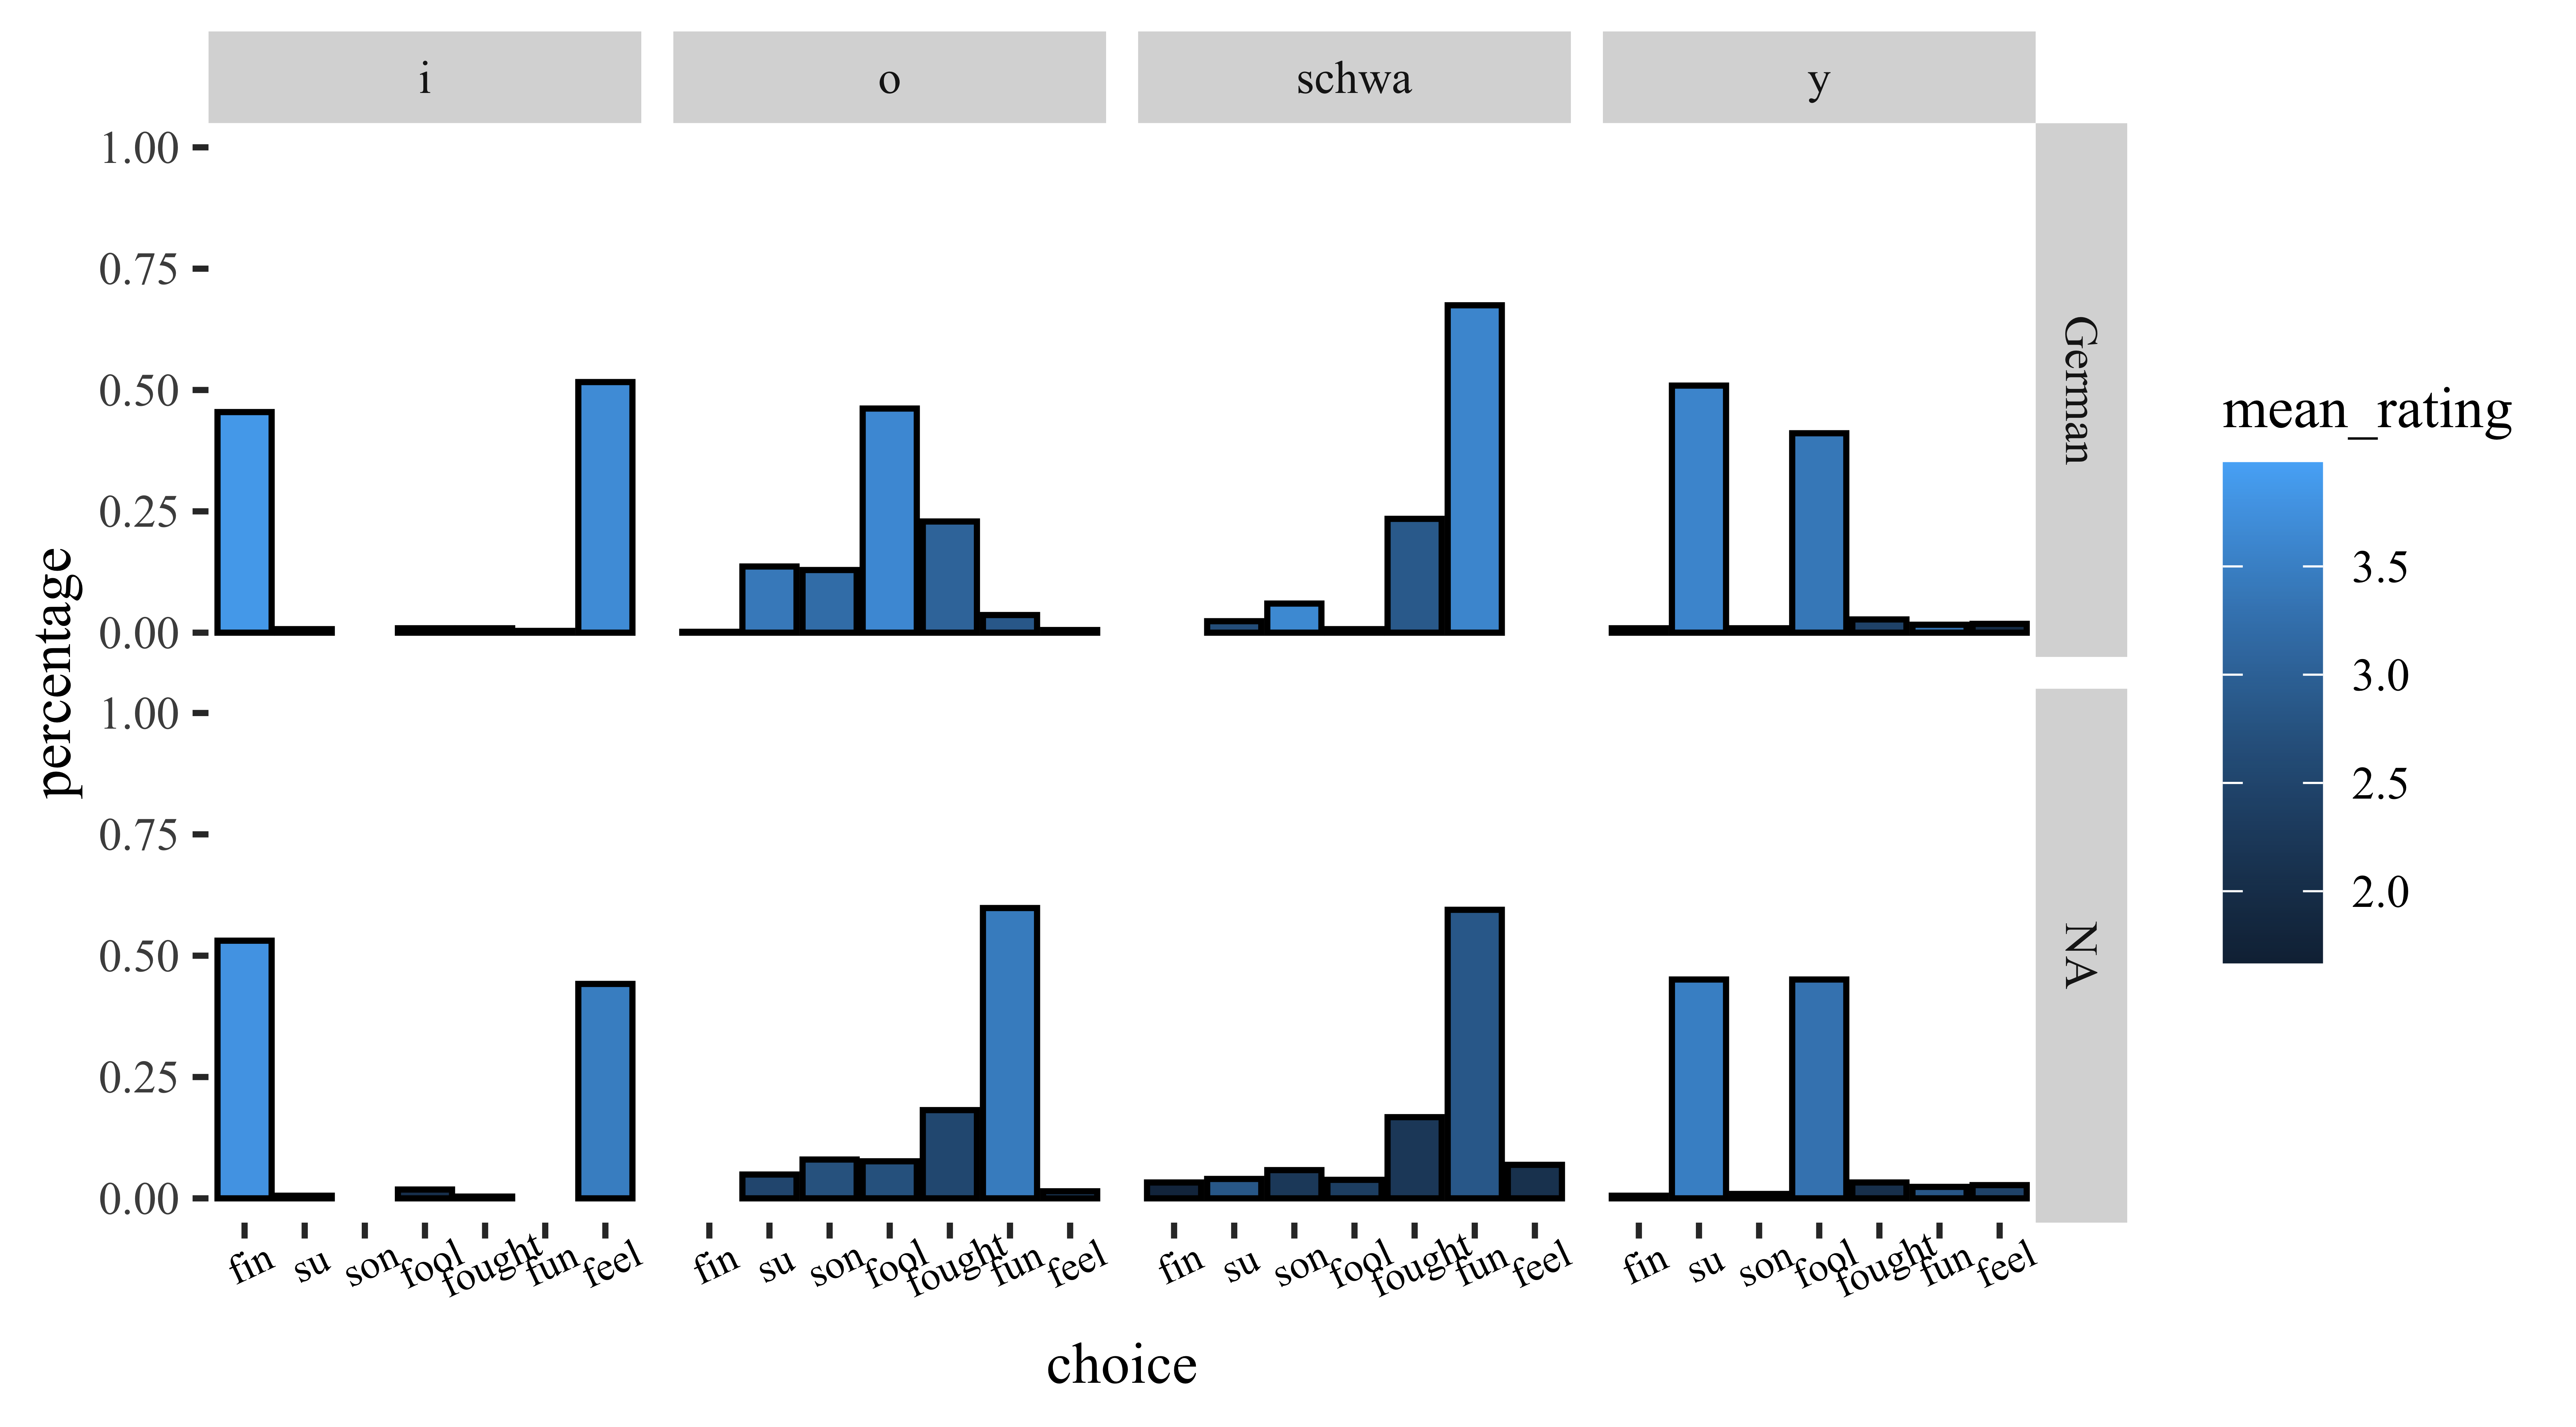
\includegraphics[width=13.5cm]{figs/eng_desc_plot.png}
\end{adjustwidth}
\caption{Self-rated L2 Proficiency. The top panels refer to the L1 of the participant and the ratings refer to their L2 (\textbf{a}) Self-rated perceptual ability (\textbf{b}) Self-reported spoken proficiency.\label{eng_desc}}
\end{figure}

\begin{table}[H] 
\caption{The percentage of categorizations of French phonemes in the English L1 group.\label{el1_fr}}
\newcolumntype{C}{>{\centering\arraybackslash}X}
\begin{tabularx}{\textwidth}{CCCCC}
\toprule
choice & i & o & schwa & y \\ 
  \hline
feel & \textbf{0.44} & 0.01 & 0.07 & 0.03 \\ 
fin & \textbf{0.53} & - & 0.03 & 0.01 \\ 
fool & 0.02 & 0.08 & 0.04 & \textbf{0.45} \\ 
fought & - & 0.18 & 0.17 & 0.03 \\ 
fun & - & \textbf{0.60} & \textbf{0.59} & 0.02 \\ 
son & - & 0.08 & 0.06 & 0.01 \\ 
su & 0.01 & 0.05 & 0.04 & \textbf{0.45} \\ 

\bottomrule
\end{tabularx}
\end{table}
\unskip

\begin{table}[H] 
\caption{The percentage of categorizations of German phonemes in the English L1 group.\label{el1_ger}}
\newcolumntype{C}{>{\centering\arraybackslash}X}
\begin{tabularx}{\textwidth}{CCCCC}
\toprule
choice & i & o & y & schwa \\ 
  \hline
feel & \textbf{0.52} & 0.01 & 0.02 &  \\ 
fin & \textbf{0.45} & 0.00 & 0.01 &  \\ 
fool & 0.01 & \textbf{0.46} & \textbf{0.41} & 0.01 \\ 
fought & 0.01 & 0.23 & 0.03 & 0.23 \\ 
fun & 0.00 & 0.04 & 0.02 & \textbf{0.67} \\ 
son & - & 0.13 & 0.01 & 0.06 \\ 
su & 0.01 & 0.14 & \textbf{0.51} & 0.02 \\ 
\bottomrule
\end{tabularx}
\end{table}
\unskip

As can be seen in Tables \ref{el1_fr} and \ref{el1_ger}, the English L1 group, given the L3 French phoneme /i/, chose both their English category /i/ provided in the choice \emph{feel} and their Spanish category /i/ provided in fin \emph{fin}.
German /i/ was categorized similarly.
For /o/ and, this group chose \emph{fun} the most often in both cases in French, while the most chosen word in German for /o/ was \emph{fool}.
The wedge in both French in German was most often assimilated to the intended category \emph{fun}
Finally, both the L3 French and German phonemes /y/ resulted in choices of \emph{fool} and \emph{su}, the English and Spanish categories for /u/.

\hypertarget{spanish-l1-group}{%
\subsection{Spanish L1 group}\label{spanish-l1-group}}

Figure \ref{span_desc} shows the percentage that each answer choice was chosen given a particular phoneme in each language.

\begin{figure}[H]
\begin{adjustwidth}{-\extralength}{0cm}
\centering
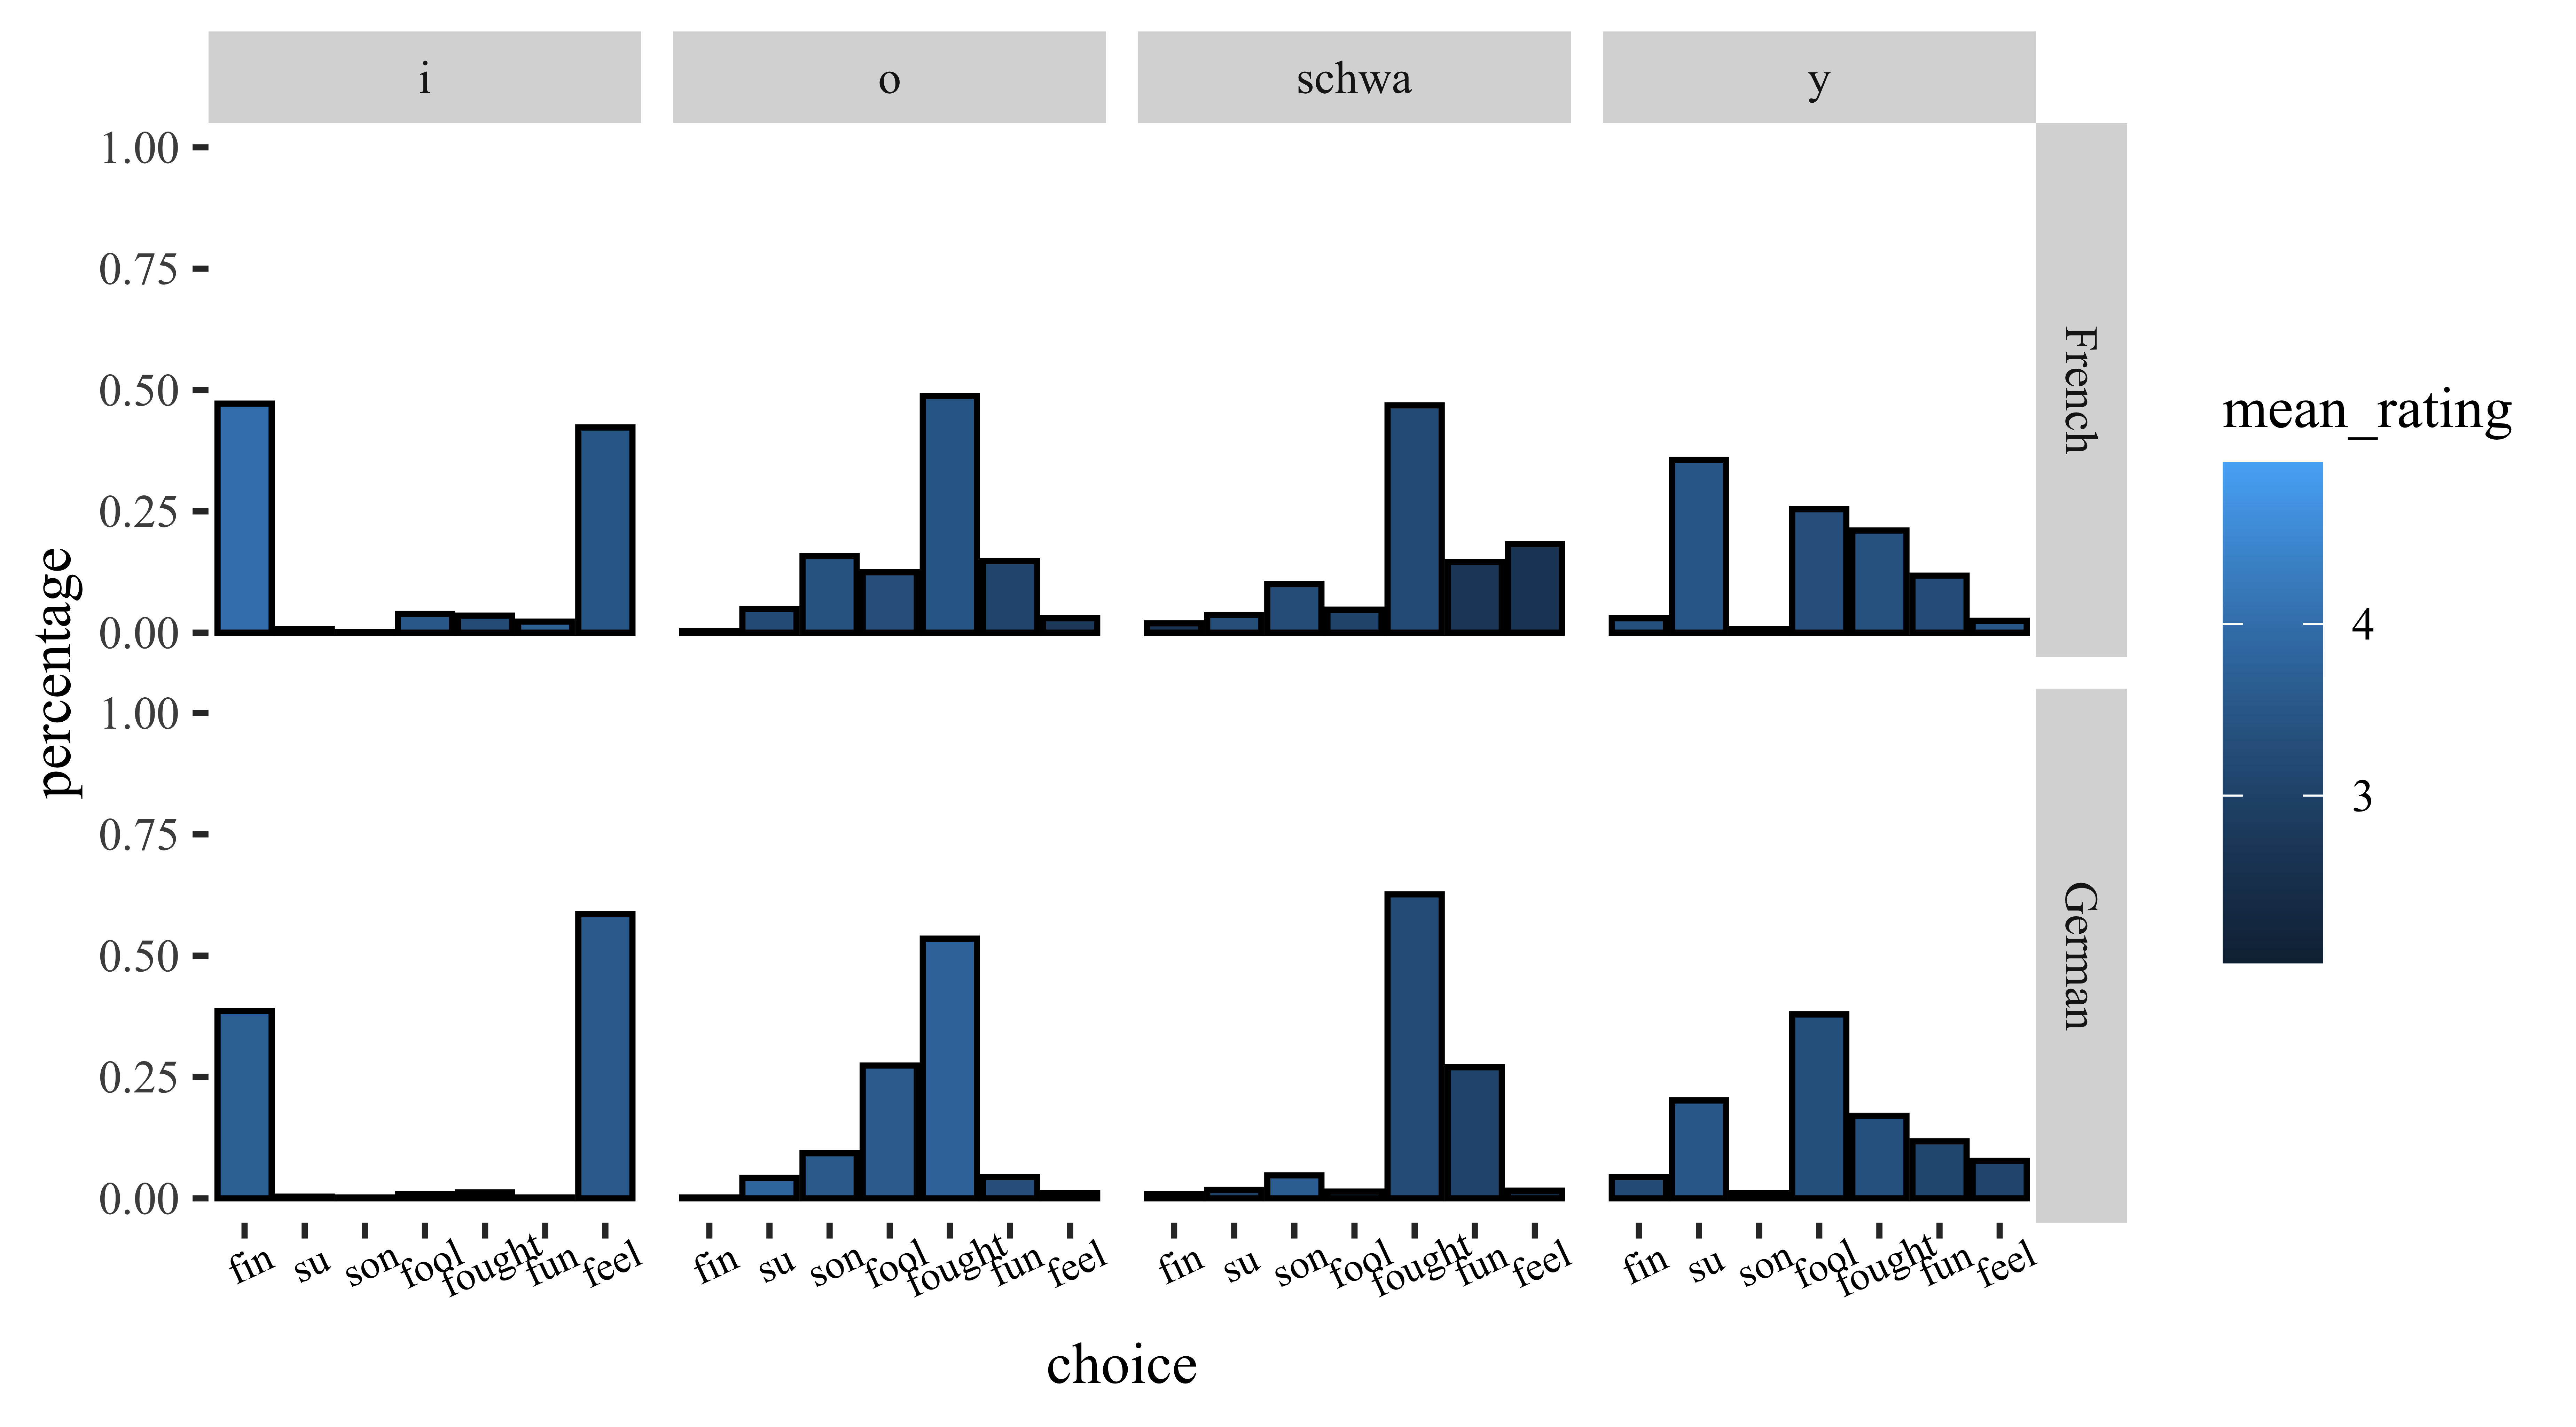
\includegraphics[width=13.5cm]{figs/span_desc_plot.png}
\end{adjustwidth}
\caption{Self-rated L2 Proficiency. The top panels refer to the L1 of the participant and the ratings refer to their L2 (\textbf{a}) Self-rated perceptual ability (\textbf{b}) Self-reported spoken proficiency.\label{span_desc}}
\end{figure}

\begin{table}[H] 
\caption{The percentage of categorizations of French phonemes in the Spanish L1 group.\label{sl1_fr}}
\newcolumntype{C}{>{\centering\arraybackslash}X}
\begin{tabularx}{\textwidth}{CCCCC}
\toprule
choice & i & o & schwa & y \\ 
  \hline
feel & \textbf{0.42} & 0.03 & 0.18 & 0.02 \\ 
fin & \textbf{0.47} & 0.00 & 0.02 & 0.03 \\ 
fool & 0.04 & 0.12 & 0.05 & 0.25 \\ 
fought & 0.04 & \textbf{0.49} & \textbf{0.47} & 0.21 \\ 
fun & 0.02 & 0.15 & 0.15 & 0.12 \\ 
son & 0.00 & 0.16 & 0.10 & 0.01 \\ 
su & 0.01 & 0.05 & 0.04 & \textbf{0.36} \\ 

\bottomrule
\end{tabularx}
\end{table}
\unskip

\begin{table}[H] 
\caption{The percentage of categorizations of German phonemes in the Spanish L1 group.\label{sl1_ger}}
\newcolumntype{C}{>{\centering\arraybackslash}X}
\begin{tabularx}{\textwidth}{CCCCC}
\toprule
choice & i & o & schwa & y \\ 
  \hline
feel & \textbf{0.59} & 0.01 & 0.02 & 0.08 \\ 
fin & \textbf{0.39} & 0.00 & 0.01 & 0.04 \\ 
fool & 0.01 & 0.27 & 0.01 & \textbf{0.38} \\ 
fought & 0.01 & \textbf{0.54} & \textbf{0.63} & 0.17 \\ 
fun & 0.00 & 0.04 & 0.27 & 0.12 \\ 
son & 0.00 & 0.09 & 0.05 & 0.01 \\ 
su & 0.00 & 0.04 & 0.02 & 0.20 \\ 

\bottomrule
\end{tabularx}
\end{table}
\unskip

Table \ref{sl1_fr} and Table \ref{sl1_ger} similarly report the percentage of each answer choice given a particular phoneme in each language in the Spanish L1 group.
The Spanish L1 group had a similar preference to the English L1 group in their categorization of /i/, where both English and Spanish categories were chosen.
However, the Spanish L1 group chose the English category given a German stimulus more often than the Spanish category.\\
In both French and German, when both /o/ and the wedge were played, the most chosen answer was \emph{fought}.
Finally, given the phoneme /y/, the Spanish L1 group chose they English \emph{fool} most often in German, and the Spanish \emph{su} most often in French.

\hypertarget{results-of-the-models}{%
\subsection{Results of the models}\label{results-of-the-models}}

The Bayesian multinomial regression models provided an inferential framework which allows for the quantification of uncertainty and avoids the pitfalls of the over-reliance on so-called ``statistical significance''.
The output of each model was converted from log-odds to probability using a combination of the \texttt{conditional\_effects} and \texttt{make\_conditions} functions in the R package \texttt{brms} (\emph{cite}).
Thus, for each phoneme in each language, the sum of the probability of choosing the categories combined is 1.
Figure \ref{i_mod} shows the probability of each choice in French and German by both groups when /i/ was the phoneme.
Figure \ref{o_mod}, shows the same set of probabilities when /o/ is played.
Figures \ref{schwa_mod} and \ref{y_mod} represent the probabilities of each response when the wedge and /y/ are played respectively.

\begin{figure}[H]
\begin{adjustwidth}{-\extralength}{0cm}
\centering
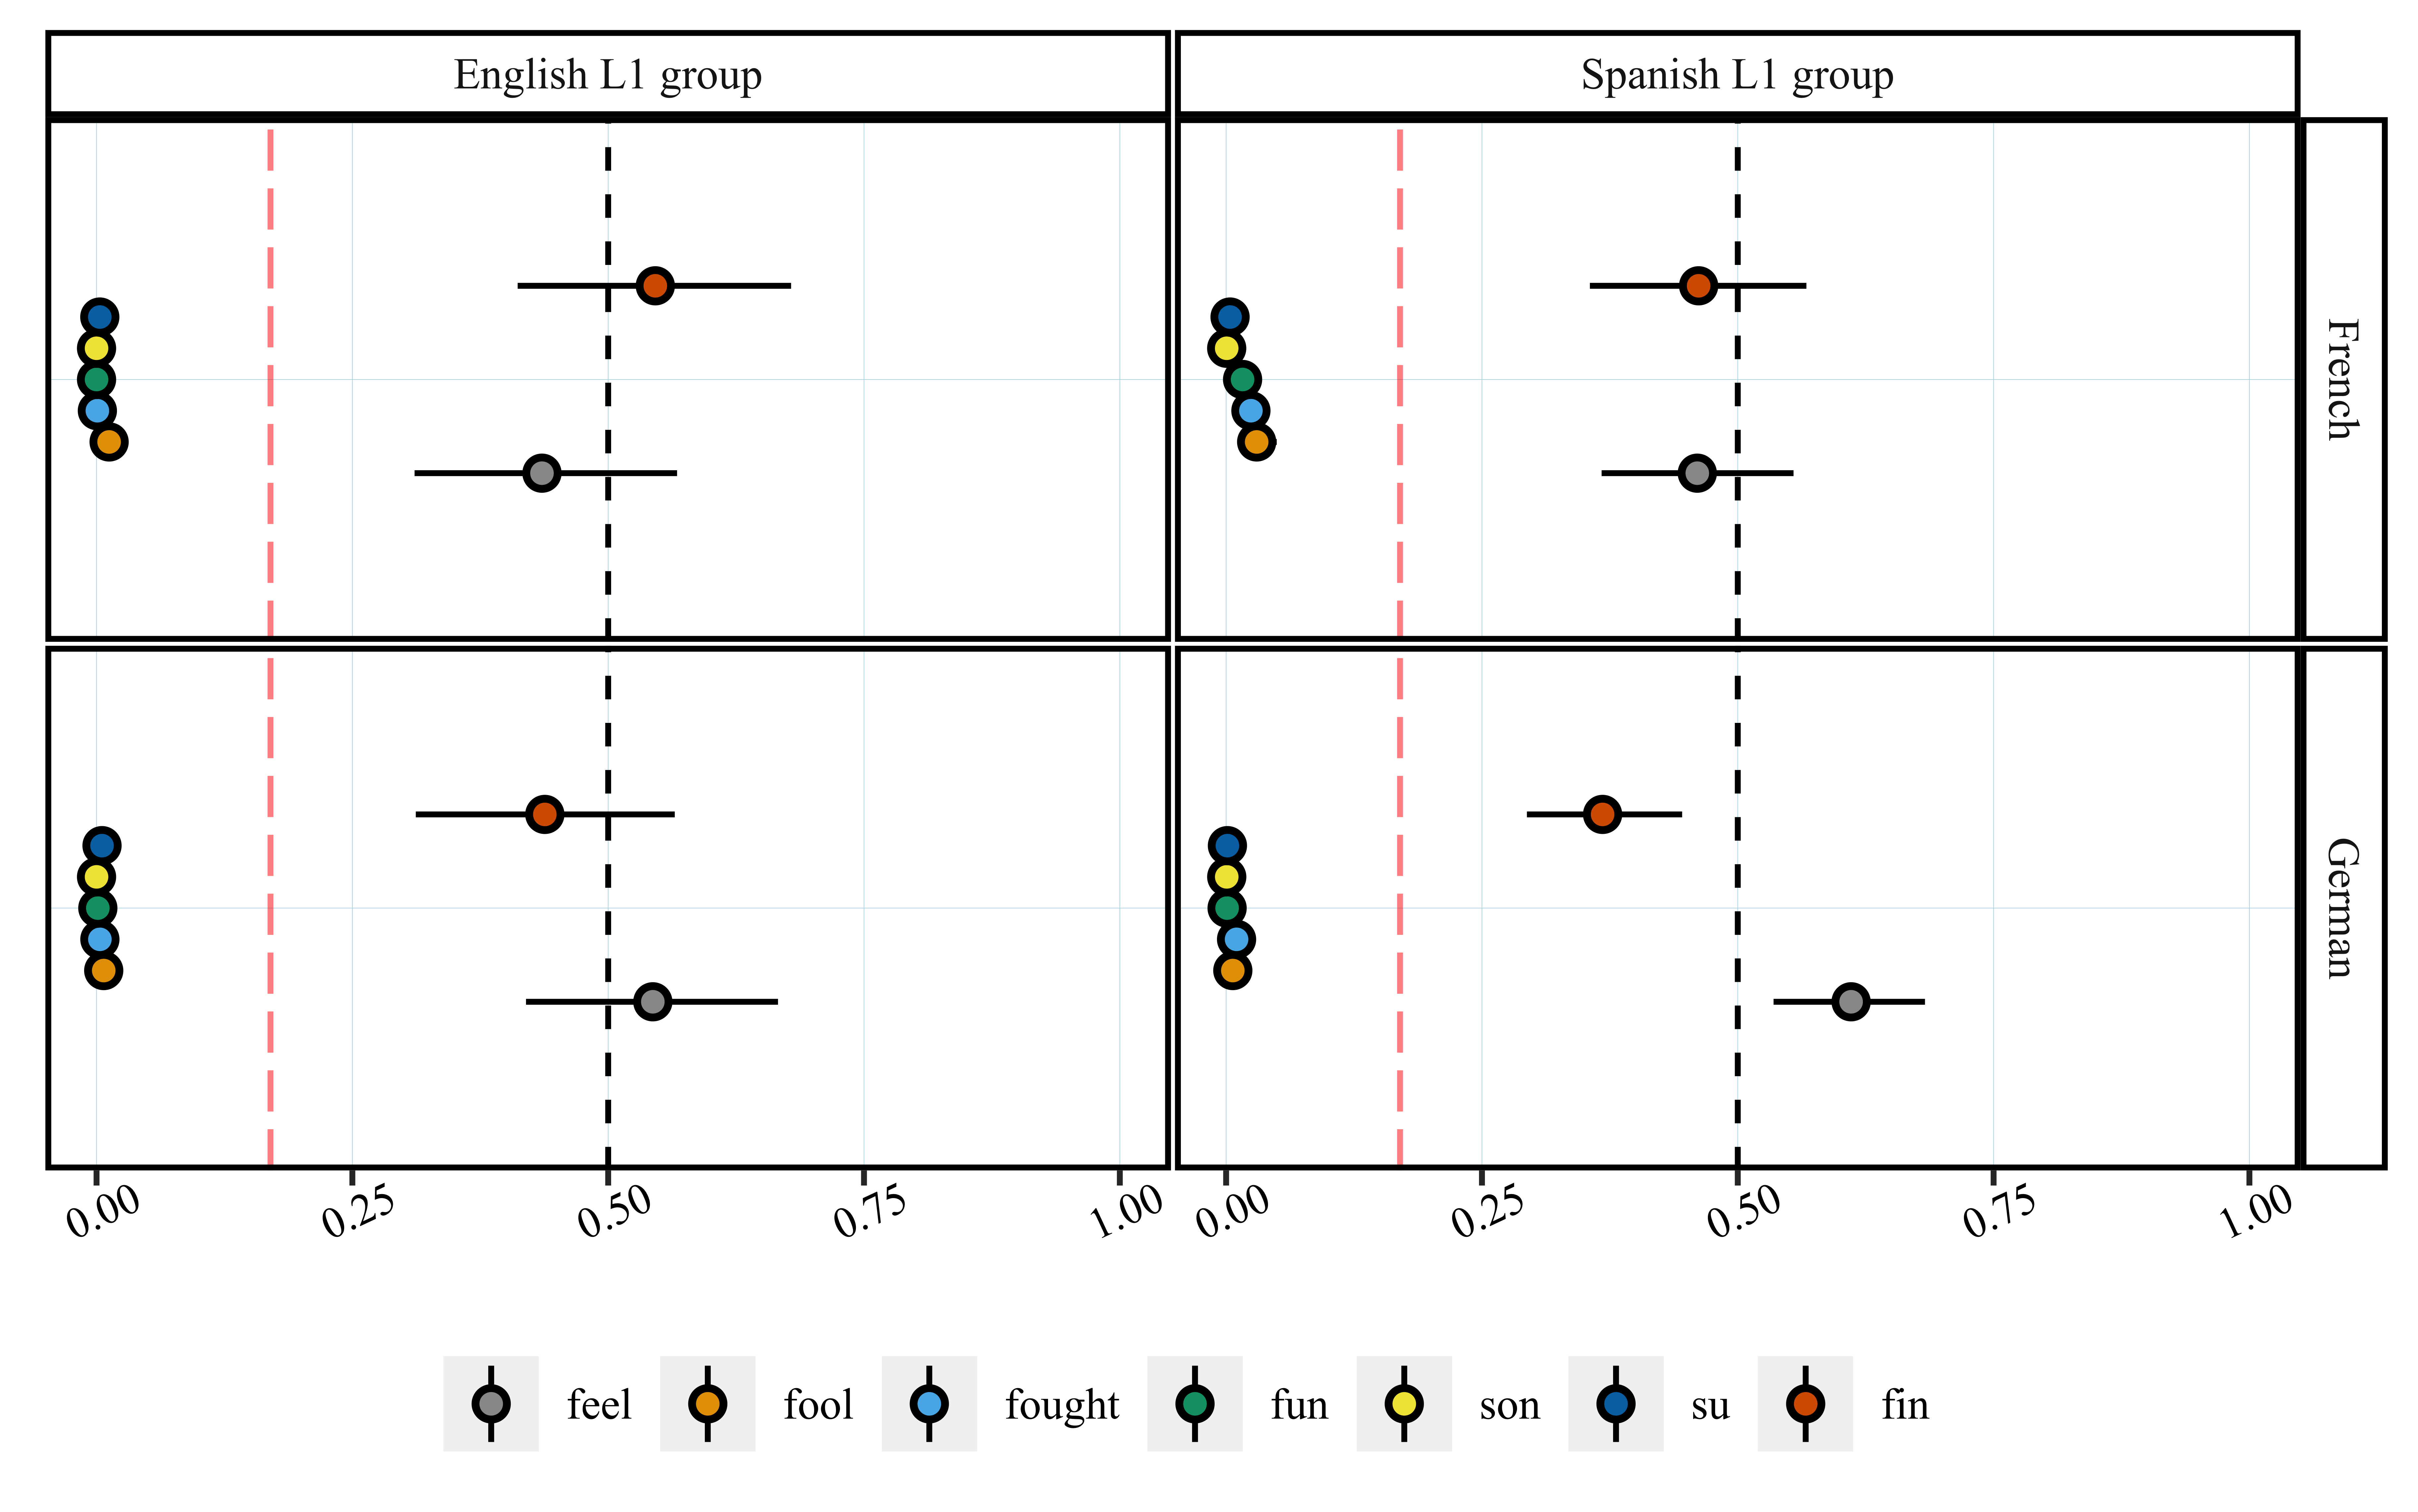
\includegraphics[width=13.5cm]{figs/i_full.png}
\end{adjustwidth}
\caption{The probability of each answer choice given the phoneme /i/ \label{i_mod}}
\end{figure}

Figure \ref{i_mod} corroborates the trends observed in the descriptive statistics when the participants in both groups were asked to categorize the phoneme /i/ in French and German.
In particular, for the English L1 group in both French and German and the Spanish L1 group in French, portions of the credible parameter estimates from the posterior distribution overlap with a probability of .5, suggesting that compelling evidence is not present for a preference for the English or Spanish category.
Differently, the Spanish L1 group did show evidence in German of a preference for the English category \emph{feel}, in which the probability of picking \emph{feel} when the stimulus was German was 0.61 (HDI = 0.53 - 0.68).
On the other hand, when phoneme was /i/ in French the probability of choosing \emph{feel} was 0.46 (HDI = 0.37 - 0.55).

\begin{figure}[H]
\begin{adjustwidth}{-\extralength}{0cm}
\centering
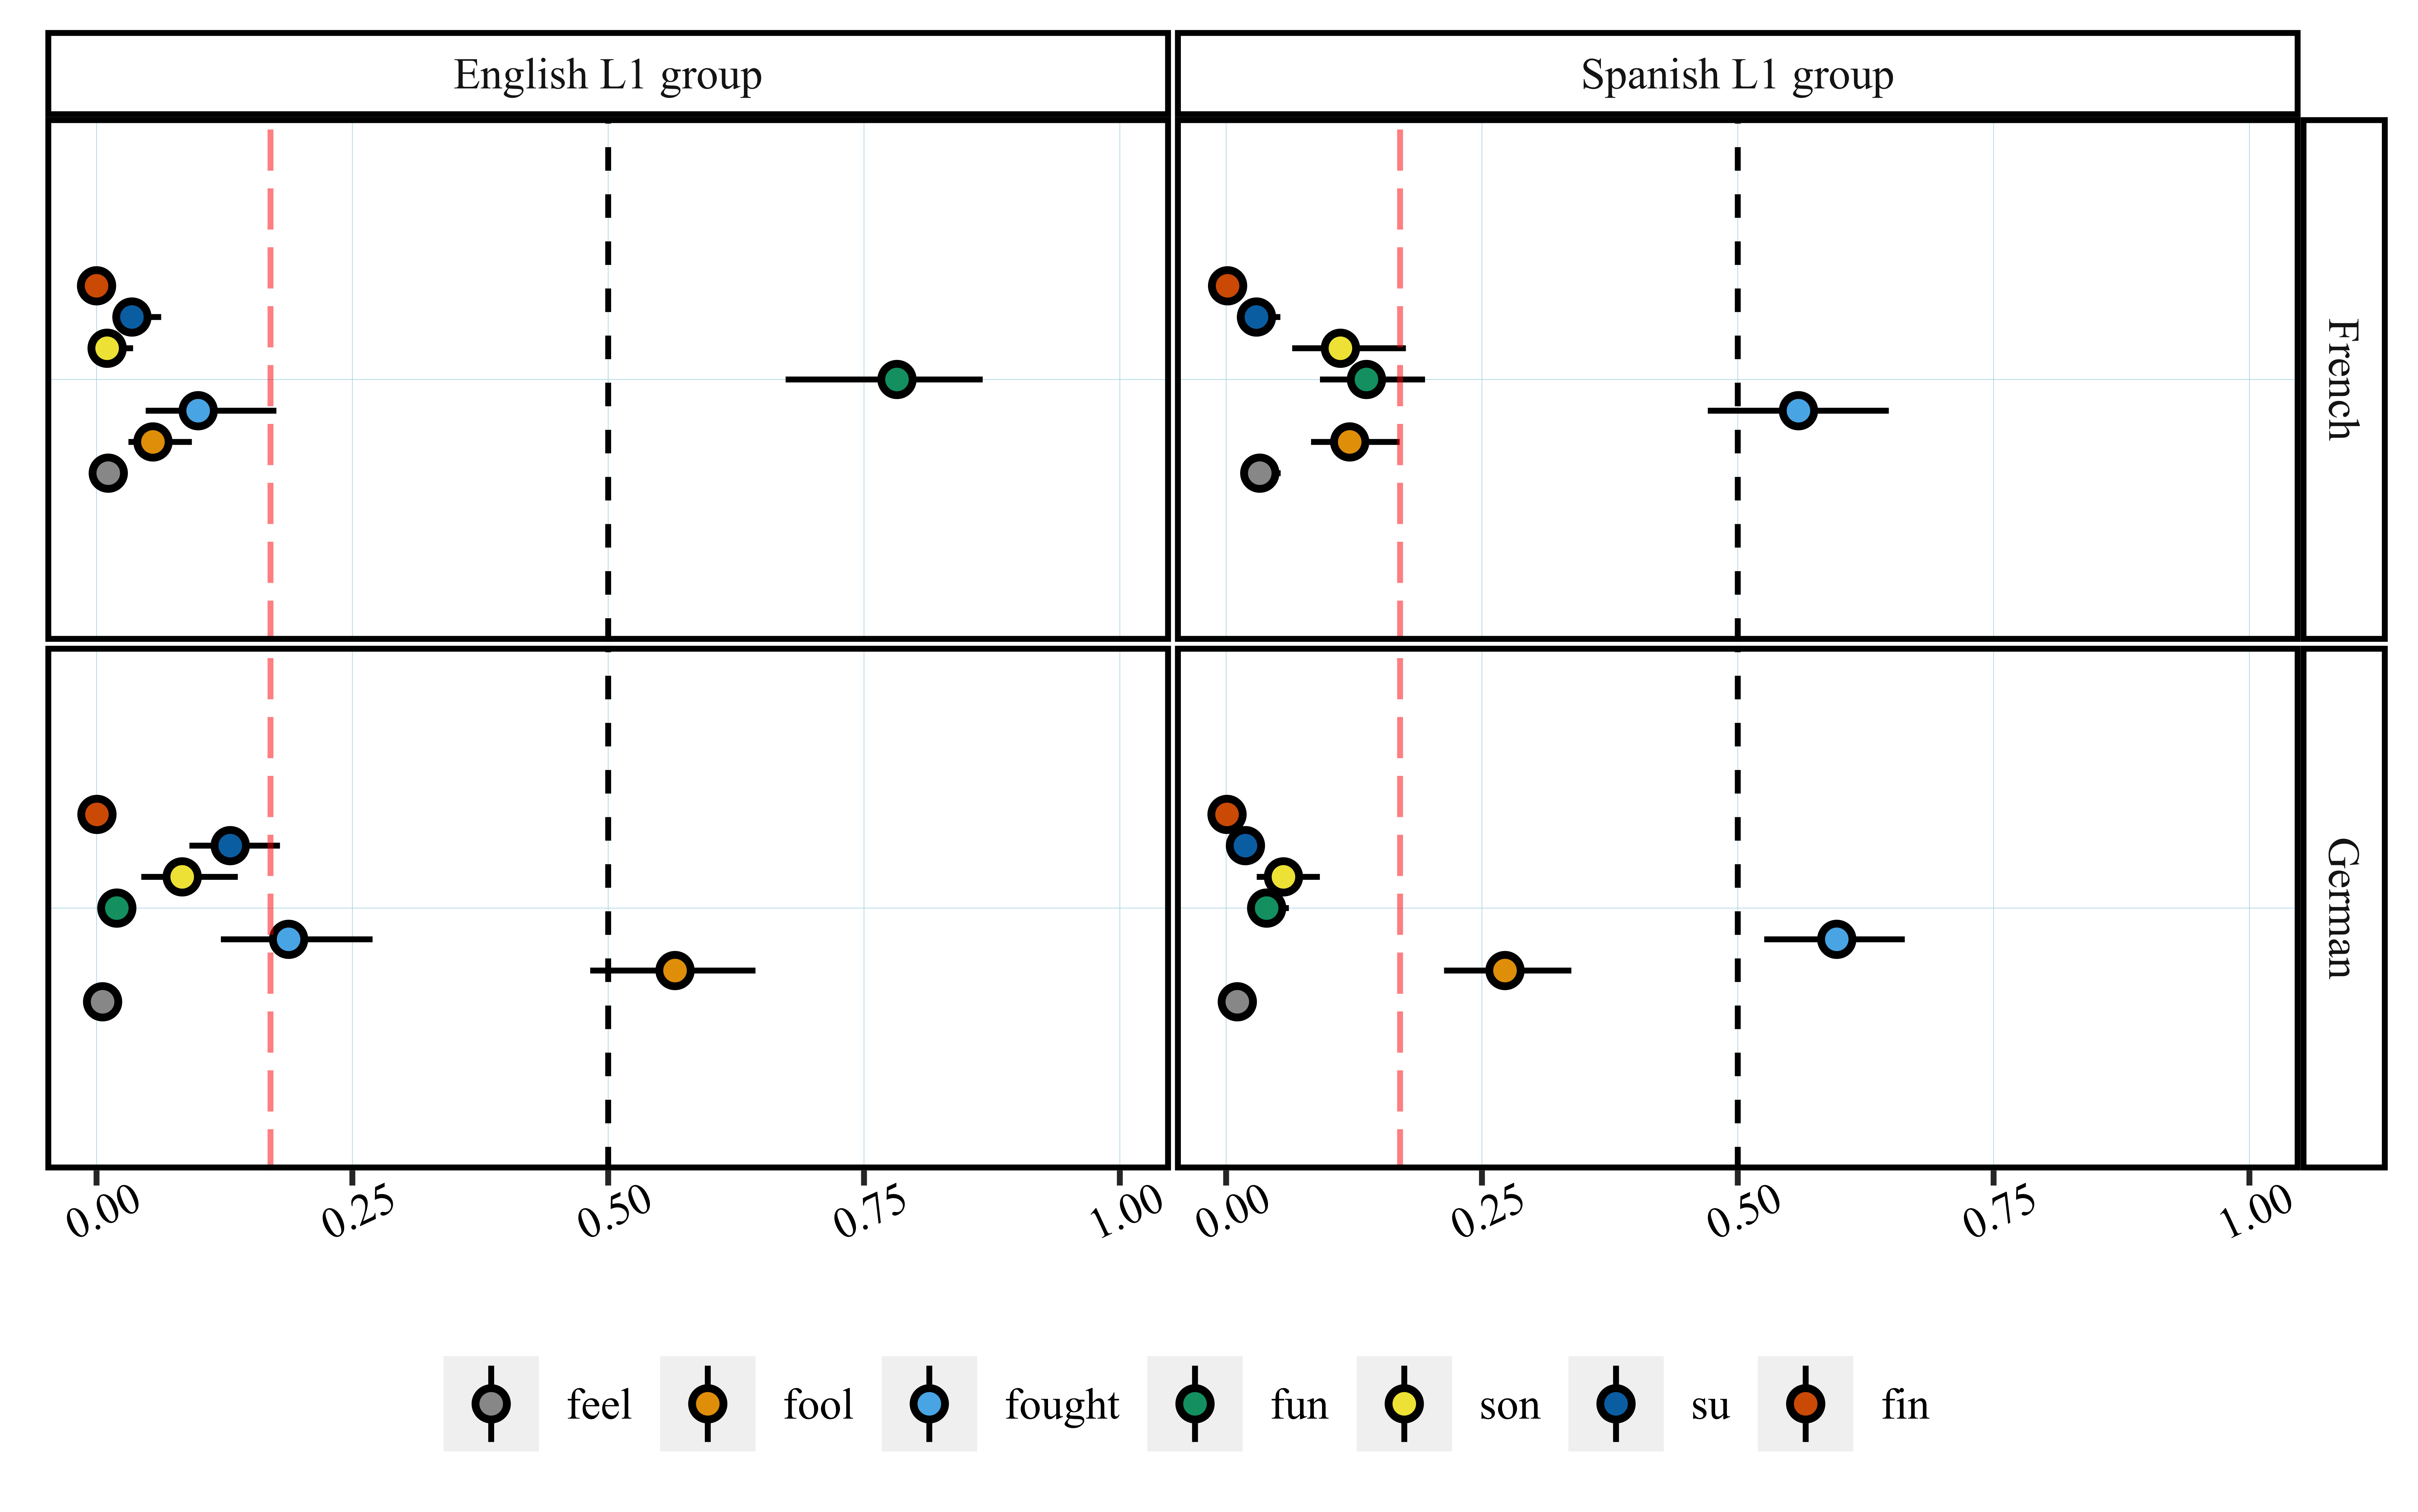
\includegraphics[width=13.5cm]{figs/o_full.png}
\end{adjustwidth}
\caption{The probability of each answer choice given the phoneme /o/ \label{o_mod}}
\end{figure}

Figure \ref{o_mod} shows the probability of each categorization of the phoneme /o/ in French and German by both groups.
The English L1 group preferred the choice \emph{fun} in French (0.78 (HDI = 0.67 - 0.87), and \emph{fool} (0.57 (HDI = 0.48 - 0.64) in German, and the Spanish L1 group preferred \emph{fought} in both languages.

\begin{figure}[H]
\begin{adjustwidth}{-\extralength}{0cm}
\centering
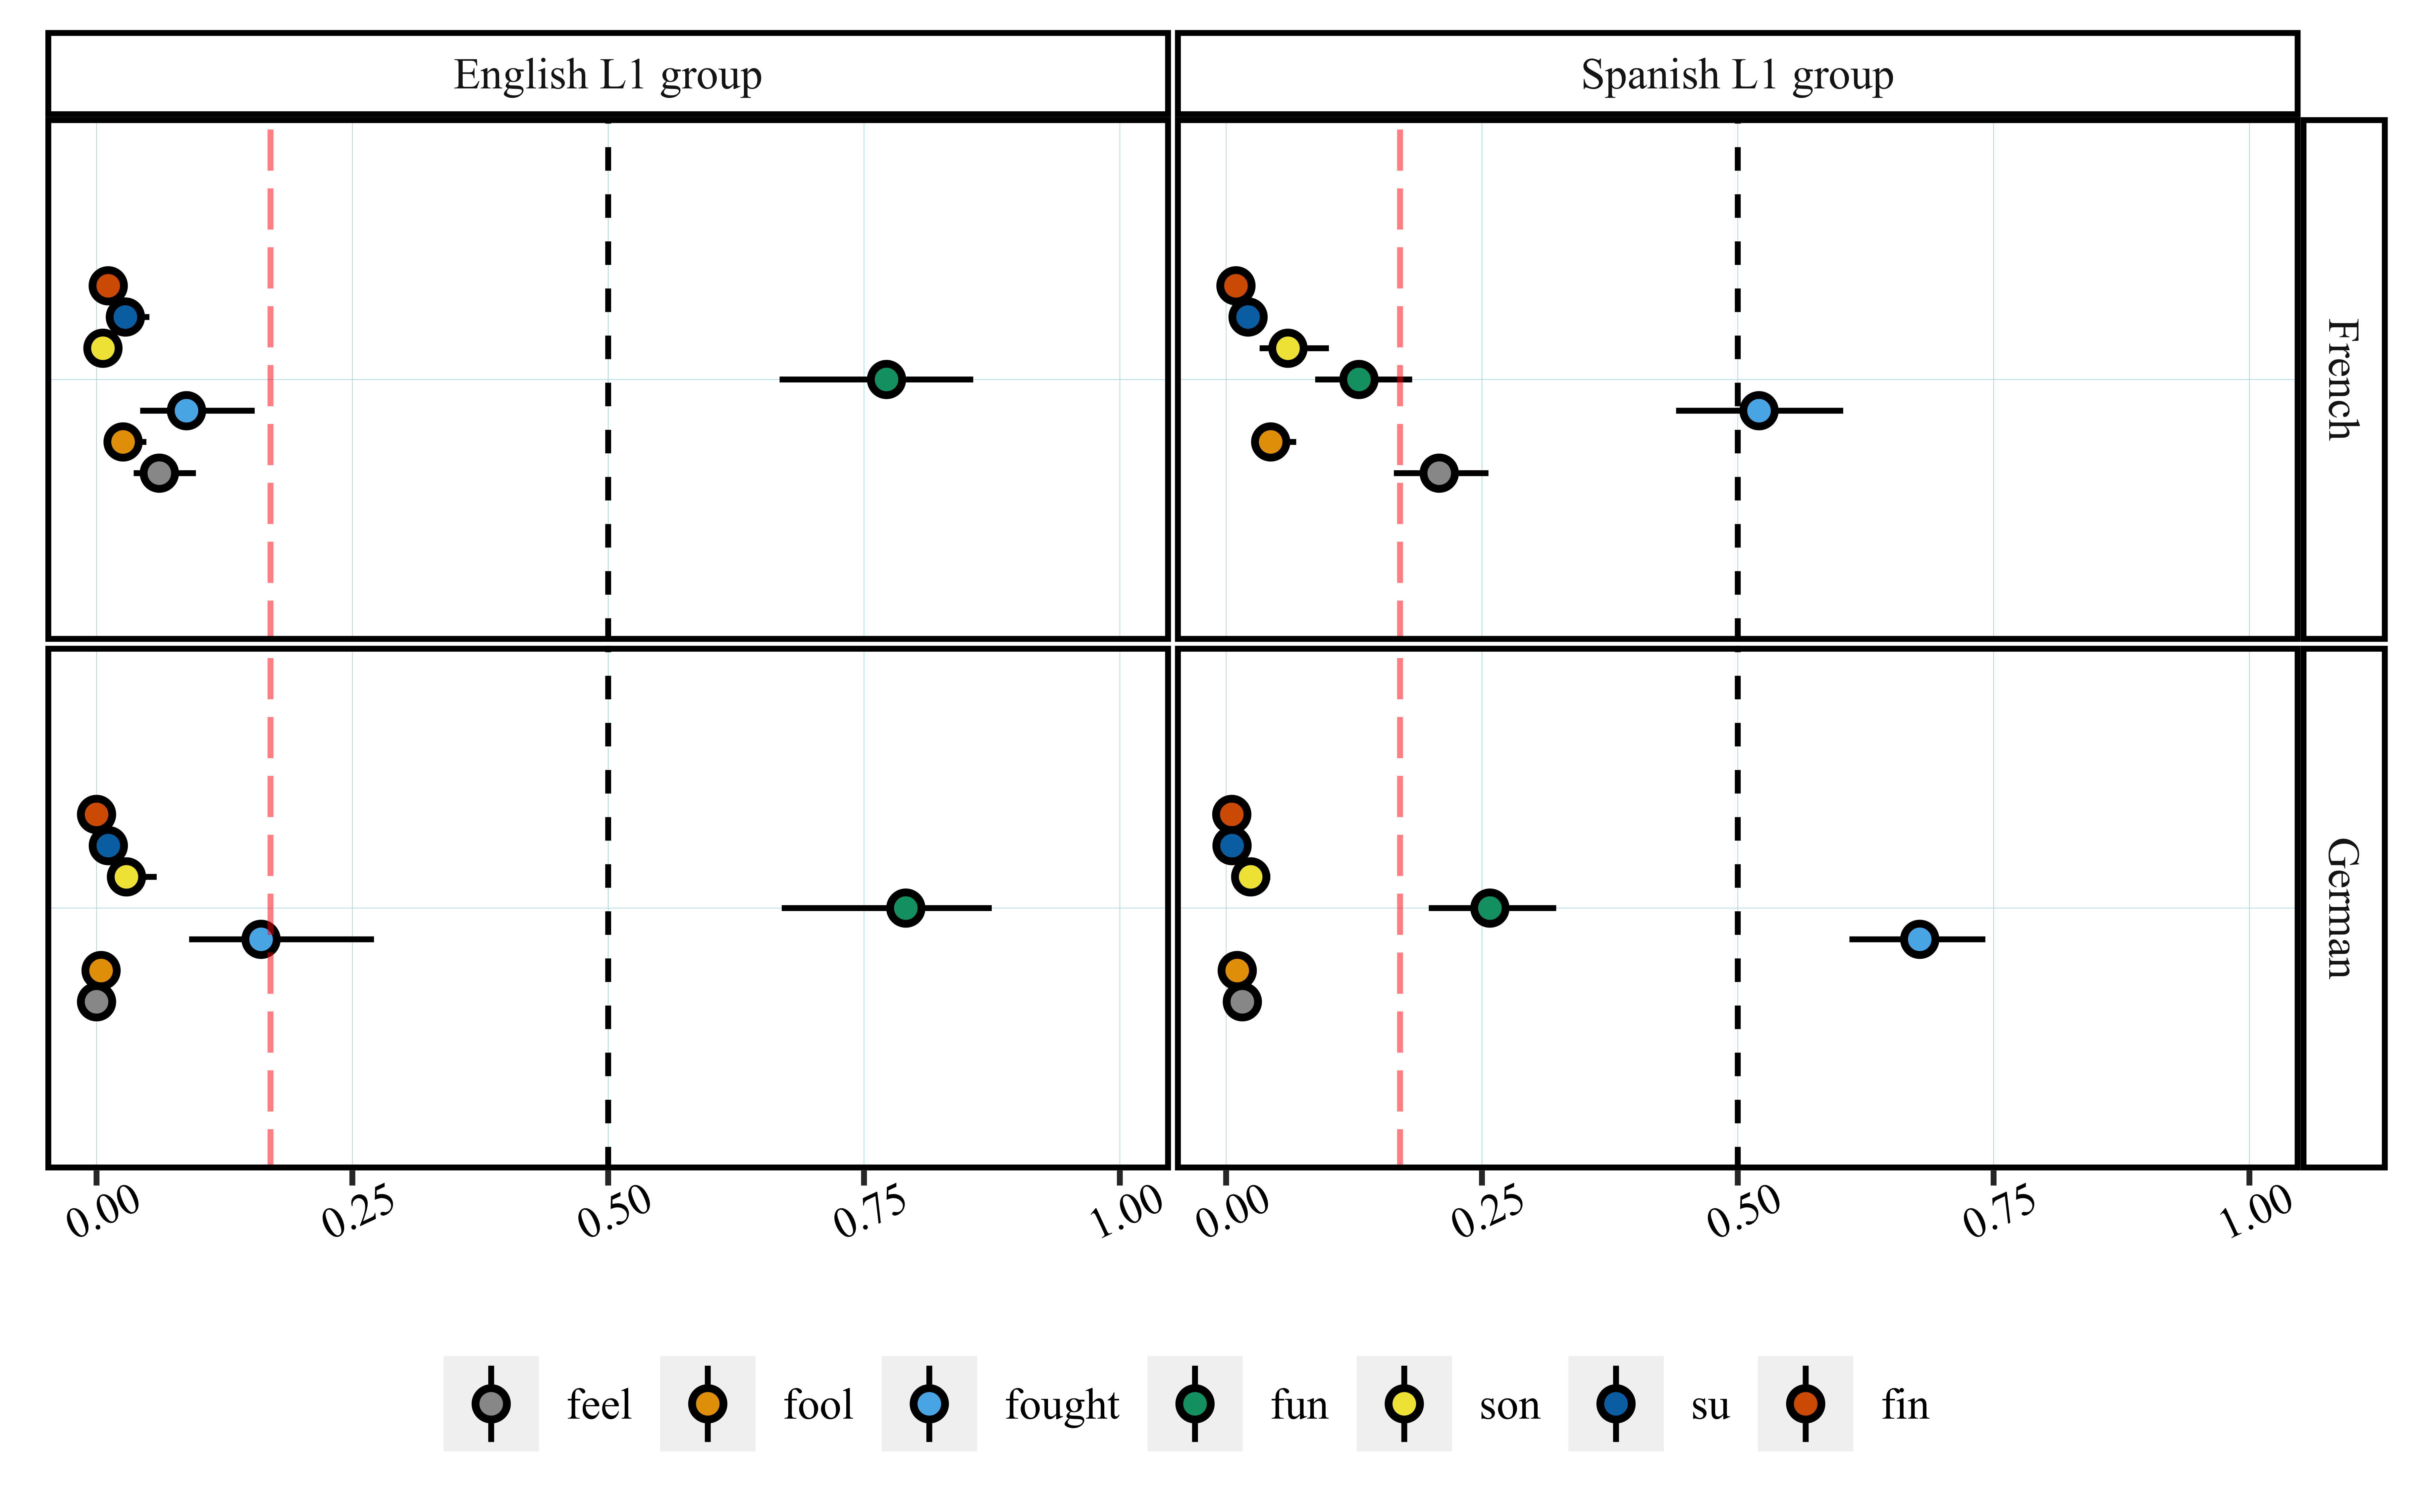
\includegraphics[width=13.5cm]{figs/schwa_full.png}
\end{adjustwidth}
\caption{The probability of each answer choice given the phoneme schwa \label{schwa_mod}}
\end{figure}

Figure \ref{schwa_mod} shows the probability of each categorization of the wedge in French and German by both groups.
The English L1 group preferred the choice \emph{fun} in both French (0.78 {[}HDI = 0.67 - 0.87{]} and German (0.79 {[}HDI = 0.67 - 0.87{]}. The Spanish L1 group preferred \emph{fought} in both languages. (French: 0.52 {[}HDI = 0.44 - 0.6{]}; German: 0.68 {[}HDI = 0.61 - 0.74{]}

\begin{figure}[H]
\begin{adjustwidth}{-\extralength}{0cm}
\centering
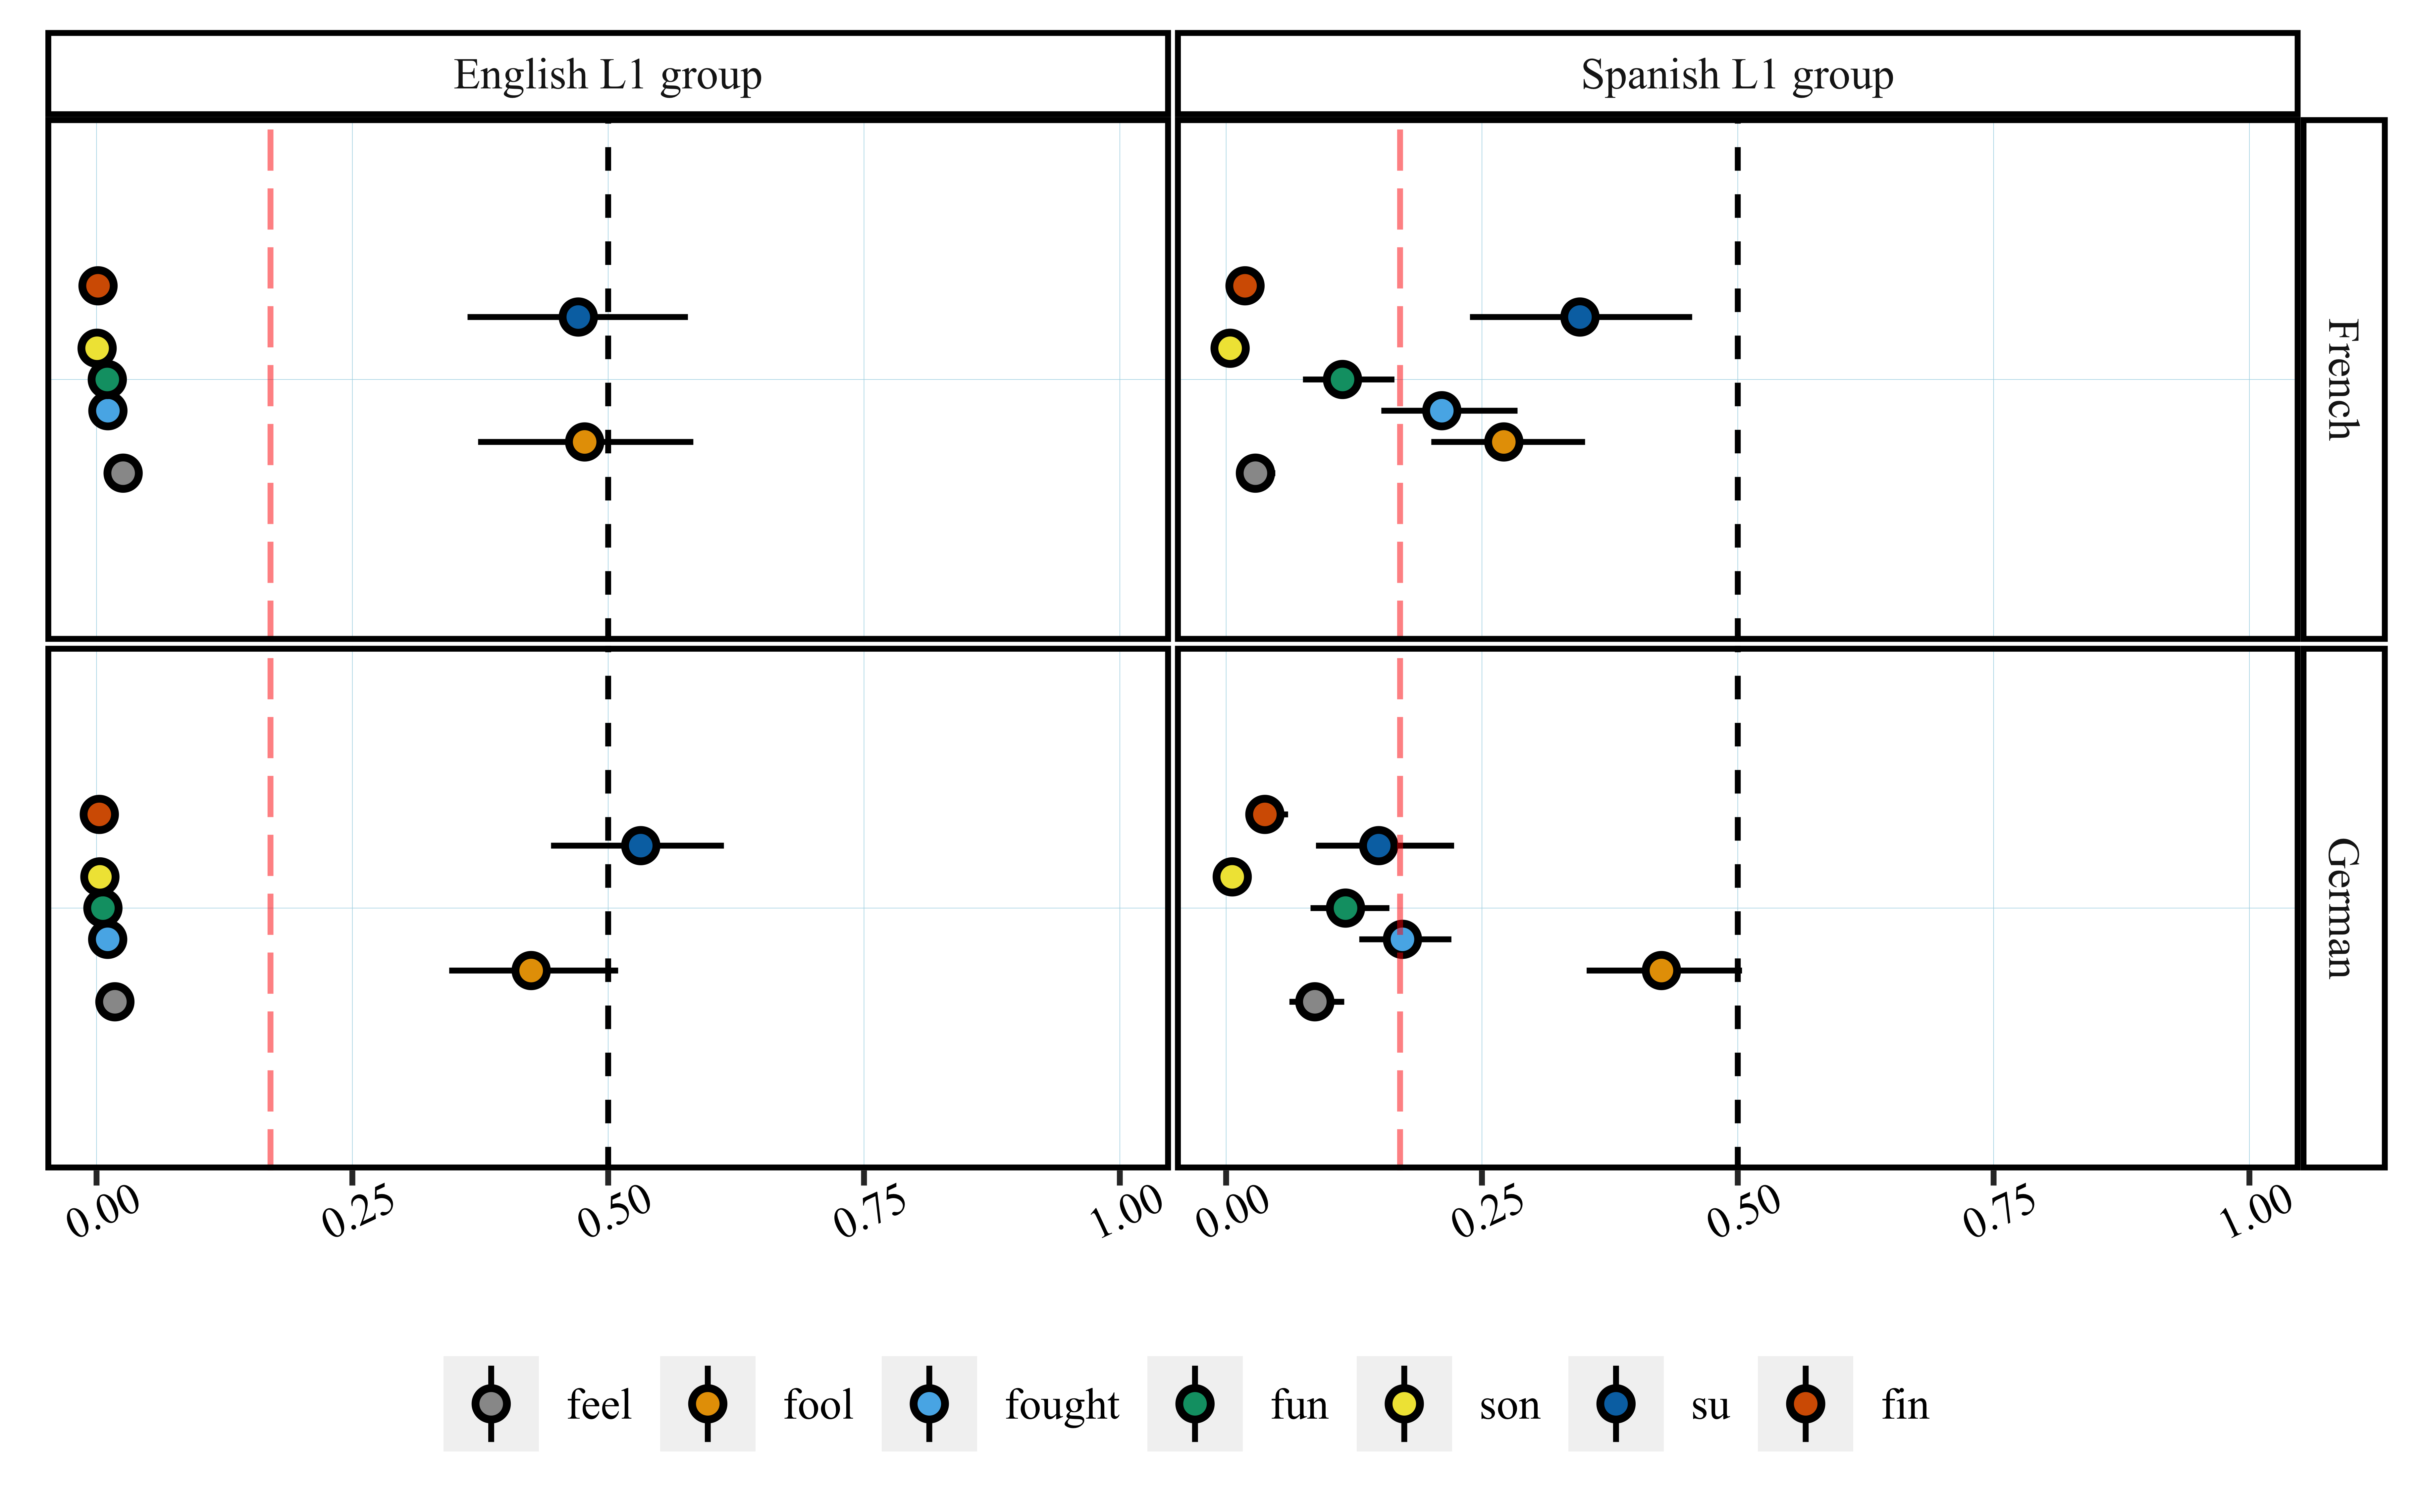
\includegraphics[width=13.5cm]{figs/y_full.png}
\end{adjustwidth}
\caption{The probability of each answer choice given the phoneme /y/ \label{y_mod}}
\end{figure}

Figure \ref{y_mod} shows the probability of each categorization of /y/ in French and German by both groups.
The English L1 group assimilated the /y/ in both French and German to their English and Spanish /u/ (choices \emph{su} and \emph{fool}), without a clear preference for either.
Probability of the English L1 group's choice of \emph{su} given the phoneme /y/ and the stimulus language German: 0.53 {[}HDI = 0.44 - 0.61{]}.
Probability of the English L1 group's choice of \emph{fool} given the phoneme /y/ and the stimulus language German: 0.42 {[}HDI = 0.34 - 0.51{]}
Probability of the English L1 group's choice of \emph{su} given the phoneme /y/ and the stimulus language French: 0.47 {[}HDI = 0.36 - 0.58{]}.
Probability of the English L1 group's choice of \emph{fool} given the phoneme /y/ and the stimulus language French: 0.48 {[}HDI = 0.37 - 0.58{]}

The Spanish L1 group, on the other hand, assimilated French /y/ to the Spanish \emph{su}, and the German /y/ to English \emph{fool}. Probability of the Spanish L1 group's choice of \emph{su} given the phoneme /y/ and the stimulus language French: 0.35 {[}HDI = 0.24 - 0.46{]}. Probability of the Spanish L1 group's choice of \emph{fool} given the phoneme /y/ and the stimulus language German: 0.43 {[}HDI = 0.35 - 0.5{]}

\section{Discussion}

The present study examined the categorization of vowel sounds in two unknown languages by Spanish-English bilinguals in both orders of acquisition.
Although there was an overall preference for English, the results suggested that bilinguals do have access to both their L1 and L2 during L3 perception and categorization.
In several instances, L3 sounds had a similar probability of being assimilated to English or Spanish sound, such as in 3 out of 4 cases with the phoneme /i/.
The results were mixed in terms of whether the L3 that the participants heard impacted their preference for English or Spanish categories.
In total, there were a three cases in which the L3 did result in the preference for an English or Spanish category out of 16 possible.
In particular, the Spanish L1 group showed a slight preference for the English /i/ (the choice \emph{feel}) when they heard /i/ in German, but not in French.
Additionally, the Spanish L1 group also categorized the phoneme /y/ differently when they heard it in L3 French than when they heard it in L3 German.
In particular, the L3 French /y/ was assimilated to Spanish /u/ (\emph{su}) and the L3 German /y/ was assimilated to English /u/ (\emph{fool}).

These results are best explained by the Linguistic Proximity Model (\citeauthor{westergaard_crosslinguistic_2017} \citeyear{westergaard_crosslinguistic_2017};
\citeauthor{westergaard_microvariation_2021} \citeyear{westergaard_microvariation_2021}), which suggests that L3 learners have access to categories in both their L1 and L2 during L3 acquisition.
On the other hand, The Typological Primacy Model (\citeauthor{rothman_typological_2010} \citeyear{rothman_typological_2010};
\citeauthor{rothman_l3_2011} \citeyear{rothman_l3_2011};
\citeauthor{baauw_cognitive_2013} \citeyear{baauw_cognitive_2013};
\citeauthor{rothman_linguistic_2015} \citeyear{rothman_linguistic_2015}) suggests that, while bilinguals have access to both their languages at first exposure, this access is lost at some point during what the model refers to as the ``initial stages'' of L3 acquisition.
While the present data does not necessarily provide counter-evidence to the TPM, it provides a starting point for future research by providing a picture of the categorization patterns of L3 phonemes in two languages by Spanish-English bilinguals which could be examined in a longitudenal design. If the TPM is correct, a distinct change in categorization would be expected to reflect a bias for a single language's category.
The present study provides a basis of comparison, and evidence that bilinguals do have access to both the L1 and L2 at first exposure.
However, in 6 our of 8 cases, global typological similarity (English and German vs.~French and Spanish), did not result in any obvious bias in categorization.

It is unclear why the Spanish L1 group seemed to be sensitive to which L3 they heard, where the English L1 group was not.
It is worth noting that there are differences between the groups in self-rated proficiency and age of onset and acquisition; the Spanish L1 group rated themselves as more proficient on average in spoken and perceptual abilities and had an earlier age of onset and acquisition on average.
The role of proficiency has been addressed in L3 models, but its precise role in influence is not yet clear.
The TPM has stated that the L2 must be sufficiently proficient to be a source of influence.
In the TPM studies to date, this has been taken to mean ``advanced proficiency''.
Though the present study was not interested in the effect of L2 proficiency on L3 categorizations, it is worth noting that the group differences in proficiency might have impacted the results, although it is difficult to say exactly how.
This notion of the impact of L2 proficiency CLI could be further investigated, in which the more traditional categorical grouping of proficiency (e.g., novice, intermediate, advanced) could also be examined in a continuous fashion and corroborated accross measures.
In other words, it's unclear for the purpose of the present study, and likely with many proficiency measures, where the TPM's cutoff for ``advanced'' should be.

The present study also had limitations.
Firstly, online studies offers unique challenges and limitations.
One potential issue is the lack of the ability to control the participant's environment outside of the instructions and experiment itself.
As a result, language mode effects (\citeauthor{grosjean1998transfer} \citeyear{grosjean1998transfer}; \citeauthor{casillas2018perceptual} \citeyear{casillas2018perceptual}) cannot be completely ruled out.
Additionally, headphone quality, speaker quality, background noise and volume level are all variables within the participant's control that could not be reasonably controlled for in the context of online data collection.
Second, self-reported proficiency, while convenient and fast, is a subjective measure of language ability that would likely be improved by a more objective proficiency measure such as the LexTALE (\citeauthor{lemhofer_introducing_2012} \citeyear{lemhofer_introducing_2012}).
While the present study did not initially hypothesize that differences in proficiency impact categorization, a look at the data suggests that this is a possibility.

\section{Conclusions}

In conclusion, the present study provided evidence for the categorization patterns of Spanish-English bilinguals at their first exposure to two distinct third languages, French and German.
It largely did not make a difference in their categorizations if bilinguals listened to stimuli in German or French, suggesting that the acoustics of the stimuli, rather than the language to which they belong, had a greater impact on categorization.
This finding has implications for L3 models, some of which suggest that L3 learners may only have access to one of their two source languages.
The present study provides a futher point of reference for future research, in which L3 model's predictinos may further be examined.

%%%%%%%%%%%%%%%%%%%%%%%%%%%%%%%%%%%%%%%%%%

%\begin{listing}[H]
%\caption{Title of the listing}
%\rule{\columnwidth}{1pt}
%\raggedright Text of the listing. In font size footnotesize, small, or normalsize. Preferred format: left aligned and single spaced. Preferred border format: top border line and bottom border line.
%\rule{\columnwidth}{1pt}
%\end{listing}


%% If the documentclass option "submit" is chosen, please insert a blank line before and after any math environment (equation and eqnarray environments). This ensures correct linenumbering. The blank line should be removed when the documentclass option is changed to "accept" because the text following an equation should not be a new paragraph.

% Example of a page in landscape format (with table and table footnote).
%\startlandscape
%\begin{table}[H] %% Table in wide page
%\caption{This is a very wide table.\label{tab3}}
%	\begin{tabularx}{\textwidth}{CCCC}
%		\toprule
%		\textbf{Title 1}	& \textbf{Title 2}	& \textbf{Title 3}	& \textbf{Title 4}\\
%		\midrule
%		Entry 1		& Data			& Data			& This cell has some longer content that runs over two lines.\\
%		Entry 2		& Data			& Data			& Data\textsuperscript{1}\\
%		\bottomrule
%	\end{tabularx}
%	\begin{adjustwidth}{+\extralength}{0cm}
%		\noindent\footnotesize{\textsuperscript{1} This is a table footnote.}
%	\end{adjustwidth}
%\end{table}
%\finishlandscape

% Example of a figure that spans the whole page width. The same concept works for tables, too.


%%%%%%%%%%%%%%%%%%%%%%%%%%%%%%%%%%%%%%%%%%

%%%%%%%%%%%%%%%%%%%%%%%%%%%%%%%%%%%%%%%%%%

%%%%%%%%%%%%%%%%%%%%%%%%%%%%%%%%%%%%%%%%%%
\vspace{6pt} 

%%%%%%%%%%%%%%%%%%%%%%%%%%%%%%%%%%%%%%%%%%
%% optional
%\supplementary{The following supporting information can be downloaded at:  \linksupplementary{s1}, Figure S1: title; Table S1: title; Video S1: title.}

% Only for the journal Methods and Protocols:
% If you wish to submit a video article, please do so with any other supplementary material.
% \supplementary{The following supporting information can be downloaded at: \linksupplementary{s1}, Figure S1: title; Table S1: title; Video S1: title. A supporting video article is available at doi: link.}

%%%%%%%%%%%%%%%%%%%%%%%%%%%%%%%%%%%%%%%%%%

\funding{This research received no external funding.}

\institutionalreview{The study was conducted in accordance with the Declaration of Helsinki, and approved by the Institutional Review Board of Rutgers University (protocol code Pro2022000193 and 2/18/22).}

\informedconsent{Informed consent was obtained from all subjects involved in the study.}

\dataavailability{The complete dataset presented in this article is openly available on Open Science Framework and can be accessed at: \url{https://osf.io/5f4zj/}} 

\acknowledgments{In this section you can acknowledge any support given which is not covered by the author contribution or funding sections. This may include administrative and technical support, or donations in kind (e.g., materials used for experiments).}

\conflictsofinterest{The authors declare no conflict of interest.} 


%%%%%%%%%%%%%%%%%%%%%%%%%%%%%%%%%%%%%%%%%%
\begin{adjustwidth}{-\extralength}{0cm}
%\printendnotes[custom] % Un-comment to print a list of endnotes

\reftitle{References}

% Please provide either the correct journal abbreviation (e.g. according to the “List of Title Word Abbreviations” http://www.issn.org/services/online-services/access-to-the-ltwa/) or the full name of the journal.
% Citations and References in Supplementary files are permitted provided that they also appear in the reference list here. 

%=====================================
% References, variant A: external bibliography
%=====================================
\externalbibliography{yes}
\bibliography{bib_lang.bib}

%=====================================
% References, variant B: internal bibliography
%=====================================


% If authors have biography, please use the format below
%\section*{Short Biography of Authors}
%\bio
%{\raisebox{-0.35cm}{\includegraphics[width=3.5cm,height=5.3cm,clip,keepaspectratio]{Definitions/author1.pdf}}}
%{\textbf{Firstname Lastname} Biography of first author}
%
%\bio
%{\raisebox{-0.35cm}{\includegraphics[width=3.5cm,height=5.3cm,clip,keepaspectratio]{Definitions/author2.jpg}}}
%{\textbf{Firstname Lastname} Biography of second author}

% For the MDPI journals use author-date citation, please follow the formatting guidelines on http://www.mdpi.com/authors/references
% To cite two works by the same author: \citeauthor{ref-journal-1a} (\citeyear{ref-journal-1a}, \citeyear{ref-journal-1b}). This produces: Whittaker (1967, 1975)
% To cite two works by the same author with specific pages: \citeauthor{ref-journal-3a} (\citeyear{ref-journal-3a}, p. 328; \citeyear{ref-journal-3b}, p.475). This produces: Wong (1999, p. 328; 2000, p. 475)

%%%%%%%%%%%%%%%%%%%%%%%%%%%%%%%%%%%%%%%%%%
%% for journal Sci
%\reviewreports{\\
%Reviewer 1 comments and authors’ response\\
%Reviewer 2 comments and authors’ response\\
%Reviewer 3 comments and authors’ response
%}
%%%%%%%%%%%%%%%%%%%%%%%%%%%%%%%%%%%%%%%%%%
\end{adjustwidth}
\end{document}
